              %******************************************%
              %                                          %
              % Modello di tesi di laurea o di dottorato %
              %            di Lorenzo Pantieri �         %
              %                                          %
              %         versione: 4 luglio 2012          %
              %                                          %
              %******************************************%
       

% I seguenti commenti speciali impostano:
% 1. utf8 come codifica di input,
% 2. PDFLaTeX come motore di composizione;
% 3. Tesi.tex come documento principale;
% 4. il controllo ortografico italiano per l'editor.

% !TEX encoding = UTF-8
% !TEX TS-program = pdflatex
% !TEX root = Tesi.tex
% !TEX spellcheck = it-IT

\documentclass[11pt,%                      % corpo del font principale
               a4paper,%                   % carta A4
%               twoside,openright,%         % fronte-retro
               oneside,openany,%           % solo fronte
               titlepage,%                 % frontespizio
               headinclude,,footinclude,%  % testatina e piede di pagina
               BCOR5mm,%                   % rilegatura di 5 mm
               cleardoublepage=empty,%     % pagine vuote senza testatina e piede di pagina
               tablecaptionabove,%         % didascalie in cima alle tabelle
               ]{scrreprt}                 % classe report di KOMA-Script;
               
\usepackage[T1]{fontenc}                   % codifica dei font:
                                           % NOTA BENE! richiede una distribuzione *completa* di LaTeX,
                                           % per esempio TeXLive o MiKTeX *complete*

\usepackage[utf8]{inputenc}                % codifica di input; anche [latin1] va bene
                                           % NOTA BENE! va accordata con le preferenze dell'editor

\usepackage[english,italian]{babel}        % per scrivere in italiano e in inglese;
                                           % l'ultima lingua (l'italiano) risulta predefinita

\usepackage[suftesi]{frontespizio}         % frontespizo
                                           % per includerlo nel documento bisogna:
                                           % 1. compilare una prima volta Tesi.tex;
                                           % 2. compilare a parte Tesi-frn.tex, generato dalla compilazione precedente;
                                           % 3. compilare ancora Tesi.tex. 

\usepackage{indentfirst}                   % rientra il primo paragrafo di ogni sezione

\usepackage{graphicx}                      % immagini

\usepackage{listings}                      % codici

\usepackage[font=small]{quoting}           % citazioni

\usepackage{amsmath,amssymb,amsthm}        % matematica

\usepackage[italian]{varioref}             % riferimenti completi della pagina

\usepackage{mparhack,fixltx2e,relsize}     % finezze tipografiche

\usepackage{tabularx}                      % tabelle di larghezza prefissata

\usepackage[style=philosophy-modern,hyperref,backref,square,natbib]{biblatex}
                                           % eccellente pacchetto per la bibliografia;
                                           % produce uno stile di citazione autore-anno; 
                                           % lo stile "numeric-comp" produce riferimenti numerici
                                          
\bibliography{Bibliografia}                % database di biblatex 
                                          
\usepackage{subfig}                        % sottofigure, sottotabelle

\usepackage{lipsum}                        % testo fittizio

\usepackage{eurosym}                       % simbolo dell'euro

\usepackage[eulerchapternumbers,%          % numeri dei capitoli nel font Euler
            subfig,%                       % se si usa il pacchetto subfig
            beramono,%                     % Bera Mono come font a spaziatura fissa
            eulermath,%                    % AMS Euler come font per la matematica
            pdfspacing,%                   % migliora il riempimento di riga
            listings,%                     % codici
%           parts,%                        % da decommentare in un documento diviso in parti
            ]{classicthesis}               % stile ClassicThesis

\usepackage{arsclassica}                   % modifica alcuni aspetti di ClassicThesis

\usepackage{bookmark}                      % segnalibri

\usepackage{acronym}

%*********************************************************************************
% impostazioni-tesi.tex
% di Lorenzo Pantieri (2011)
% file che contiene le impostazioni della tesi
%*********************************************************************************


%*********************************************************************************
% Comandi persaonali
%*******************************************************
\newcommand{\myName}{Daniele Biasini}                       % autore
\newcommand{\myTitle}{Analisi di copertura di una rete di UAV basata sull'impiego di tecnologie LTE} % titolo
\newcommand{\myDegree}{Tesi di laurea triennale}                       % tipo di tesi
\newcommand{\myUni}{Universit\`a degli Studi di Roma Tor Vergata} % universit�
\newcommand{\myFaculty}{Facolt\`a di Ingegneria}    % facolt�
\newcommand{\myDepartment}{Dipartimento di Ingegneria dell'Informazione}         % dipartimento
\newcommand{\myProf}{Franco Mazzenga}      % relatore
\newcommand{\myLocation}{Roma}                         % dove
\newcommand{\myTime}{Settembre 2012}                          % quando
%\newcommand{\uav}{\emph{UAV }}
%\newcommand{\elm}{\emph{e.m. }}
%\newcommand{\lte}{\emph{LTE }}


%*********************************************************************************
% Impostazioni di amsmath, amssymb, amsthm
%*********************************************************************************

% comandi per gli insiemi numerici (serve il pacchetto amssymb)
\newcommand{\numberset}{\mathbb} 
\newcommand{\N}{\numberset{N}} 
\newcommand{\R}{\numberset{R}} 

% un ambiente per i sistemi
\newenvironment{sistema}%
  {\left\lbrace\begin{array}{@{}l@{}}}%
  {\end{array}\right.}

% definizioni (serve il pacchetto amsthm)
\theoremstyle{definition} 
\newtheorem{definizione}{Definizione}

% teoremi, leggi e decreti (serve il pacchetto amsthm)
\theoremstyle{plain} 
\newtheorem{teorema}{Teorema}
\newtheorem{legge}{Legge}
\newtheorem{decreto}[legge]{Decreto}
\newtheorem{murphy}{Murphy}[section]



%*********************************************************************************
% Impostazioni di biblatex
%*********************************************************************************
\defbibheading{bibliography}{%
\cleardoublepage
\manualmark
\phantomsection 
\addcontentsline{toc}{chapter}{\tocEntry{\bibname}}
\chapter*{\bibname\markboth{\spacedlowsmallcaps{\bibname}}
{\spacedlowsmallcaps{\bibname}}}}



%*********************************************************************************
% Impostazioni di listings
%*********************************************************************************
\lstset{language=[LaTeX]Tex,%C++,
    keywordstyle=\color{RoyalBlue},%\bfseries,
    basicstyle=\small\ttfamily,
    %identifierstyle=\color{NavyBlue},
    commentstyle=\color{Green}\ttfamily,
    stringstyle=\rmfamily,
    numbers=none,%left,%
    numberstyle=\scriptsize,%\tiny
    stepnumber=5,
    numbersep=8pt,
    showstringspaces=false,
    breaklines=true,
    frameround=ftff,
    frame=single
} 



%*********************************************************************************
% Impostazioni di hyperref
%*********************************************************************************
\hypersetup{%
    hyperfootnotes=false,pdfpagelabels,
    %draft,	% = elimina tutti i link (utile per stampe in bianco e nero)
    colorlinks=true, linktocpage=true, pdfstartpage=1, pdfstartview=FitV,%
    % decommenta la riga seguente per avere link in nero (per esempio per la stampa in bianco e nero)
    %colorlinks=false, linktocpage=false, pdfborder={0 0 0}, pdfstartpage=1, pdfstartview=FitV,% 
    breaklinks=true, pdfpagemode=UseNone, pageanchor=true, pdfpagemode=UseOutlines,%
    plainpages=false, bookmarksnumbered, bookmarksopen=true, bookmarksopenlevel=1,%
    hypertexnames=true, pdfhighlight=/O,%nesting=true,%frenchlinks,%
    urlcolor=webbrown, linkcolor=RoyalBlue, citecolor=webgreen, %pagecolor=RoyalBlue,%
    %urlcolor=Black, linkcolor=Black, citecolor=Black, %pagecolor=Black,%
    pdftitle={\myTitle},%
    pdfauthor={\textcopyright\ \myName, \myUni, \myFaculty},%
    pdfsubject={},%
    pdfkeywords={},%
    pdfcreator={pdfLaTeX},%
    pdfproducer={LaTeX with hyperref and ClassicThesis}%
}



%*********************************************************************************
% Impostazioni di graphicx
%*********************************************************************************
\graphicspath{{Immagini/}} % cartella dove sono riposte le immagini



%*********************************************************************************
% Margini ottimizzati per l'A4
%*********************************************************************************
\areaset[current]{336pt}{750pt}
\setlength{\marginparwidth}{7em}
\setlength{\marginparsep}{2em}%



%*********************************************************************************
% Altro
%*********************************************************************************

% [...] ;-)
\newcommand{\omissis}{[\dots\negthinspace]}

% eccezioni all'algoritmo di sillabazione
\hyphenation{Fortran ma-cro-istru-zio-ne nitro-idrossil-amminico}                  % file con le impostazioni personali


\begin{document}
\pagenumbering{roman}
\pagestyle{plain}

%******************************************************************
% Materiale iniziale
%******************************************************************
\input{MaterialeInizialeFinale/Frontespizio}
%\input{MaterialeInizialeFinale/Colophon}
\input{MaterialeInizialeFinale/Dedica}
\input{MaterialeInizialeFinale/Indici}
\input{MaterialeInizialeFinale/Sommario+Abstract}
%\input{MaterialeInizialeFinale/Ringraziamenti}
\input{MaterialeInizialeFinale/Introduzione}
\pagestyle{scrheadings} 
\cleardoublepage
%******************************************************************
% Materiale principale
%******************************************************************
\pagenumbering{arabic}
\chapter{Unmanned Aerial Vehicle}
\label{cap:uav}
Con il termine \emph{Unmanned Aerial Vehicle} si intendono velivoli senza pilota, i quali possono essere pilotati da remoto
o possono volare autonomamente secondo un itinerario prestabilito. \\
Gli \ac{UAV} sono attualmente utilizzati per una serie di missioni, incluse le ricognizioni e i ruoli d'attacco; è quindi 
necessaria la distinzione dai missili. Gli \ac{UAV} sono definiti come controllabili, e mantengono un volo orizzontale 
sostenuto e alimentato da un getto o motore alternativo. Un missile può essere considerato come un \ac{UAV}, 
ma si distingue da esso poiché il veicolo è l'arma stessa. \\
La FAA ha racchiuso l'acronimo \ac{UAV} in quello più generale di \ac{UAS} riflettente il 
fatto che questo tipo di veicoli comprende sia sistemi terrestri come gli \ac{UGV} che gli \ac{UAV}. \\
L'utilizzo degli \ac{UAV} oggigiorno è diventato sempre più necessario, nel caso di operazioni militari il loro uso è ormai 
consolidato, mentre è in crescita l'utilizzo per missioni civili e non militari. \\
Il grande vantaggio è il loro impiego in quelle che sono dette missioni \emph{dull, dirty and dangerous} (noiose, sporche e 
pericolose), grazie agli \ac{UAV} infatti è possibile risparmiare risorse economiche ed umane.

\begin{figure}
  \centering
  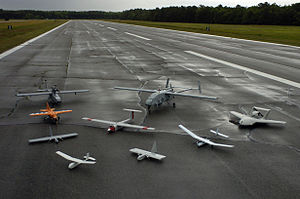
\includegraphics[height=0.25\textheight]{Immagini/gruppouav}
  \caption{Un gruppo di \ac{UAV}}
  \label{img:gruppouav}
\end{figure}

\section{Componenti}
Nonostante il nome faccia pensare ad un dispositivo indipendente, in grado di volare autonomamente, un \ac{UAV} è ben più complesso, 
esso non si riduce al solo velivolo senza pilota, ma anche ad una serie di apparecchiature che permettono il controllo da remoto.
La componentistica di un \ac{UAV} può essere divisa in due: il segmento di volo e il segmento di terra.

\begin{figure}[!h]
  \centering
  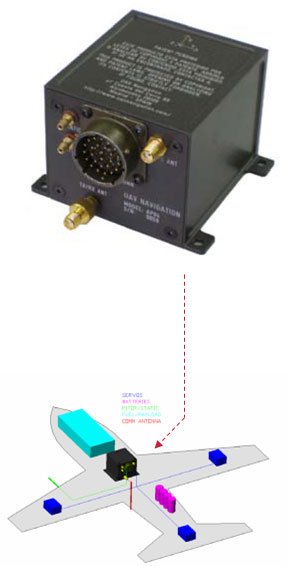
\includegraphics[height=0.25\textheight]{Immagini/segvolo}
  \caption{Componentistica interna di un \ac{UAV}.}
  \label{img:comp}
\end{figure}

\subsection*{Segmento di volo}
La gestione del volo di un \ac{UAV} può variare da modello a modello, alcuni sono in grado di decollare o atterrare autonomamente, altri,
invece, possono essere completamente gestiti da remoto. Il controllo del volo è gestito da remoto o controllato attraverso un percorso
prestabilito. \\
A bordo è presente il \emph{GN\&C} (sistema di Guida, Navigazione e Controllo), che gestisce il volo anche in assenza di segnale da terra,
inoltre a bordo possono essere presenti telecamere che mostrano immagini dall'aeromobile, anche in tempo reale; come nel caso della figura
\ref{img:vista}, l'\ac{UAV} controlla una zona agricola.

\begin{figure}
  \centering
  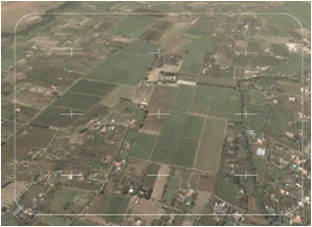
\includegraphics[height=0.25\textheight]{Immagini/segterra3}
  \caption{Vista dalla telecamera di un \ac{UAV}}
  \label{img:vista}
\end{figure}

\subsection*{Segmento di terra}
Il controllo a terra di un \ac{UAV} è costituito da:
\begin{itemize}
 \item GCS: (Ground Control System) È il controllo a terra del velivolo, svolge molte funzioni, come la rilevazione della posizione dell'
 \ac{UAV}, scambio dei dati con il velivolo, permette il pilotaggio manuale e controlla l'orientamento dell'Antenna Tracking System.
 \item Ground Computer: Permette l'elaborazione dei dati di telemetria e delle immagini inviate dall'\ac{UAV} con la telecamera a bordo.
 \item Antenna tracking system: L'uso di questo tipo di apparecchiature permette il controllo del velivolo durante il volo.
 \item Joystick: Questo strumento permette il controllo manuale del velivolo.
\end{itemize}

\begin{figure}[!h]
  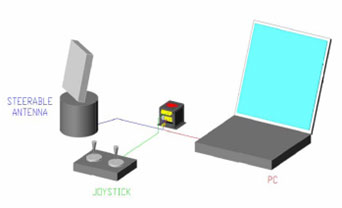
\includegraphics[height=0.25\textheight]{Immagini/segterra1}
  \caption{Apparecchiatura di terra di un \ac{UAV}.}
  \label{img:terra}
\end{figure}

\section{Impieghi tipici degli UAV}
Gli \ac{UAV}, grazie alla possibilità di essere controllati da remoto, si prestano facilmente ad utilizzi di vario tipo. \\

\subsection*{Telerilevamento}
Attraverso il telerilevamento è possibile monitorare e quindi ricavare informazioni, qualitative e quantitative, 
relative all'area coperta dall'\ac{UAV}. \\
Questo tipo di \ac{UAV} utilizza una vasta gamma di sensori come il sensore di misura dello spettro elettromagnetico, 
sensore a raggi gamma, sensori biologici e chimici. I sensori elettromagnetici includono principalmente telecamere a spettro
visivo o a infrarossi (Fig. \ref{img:infrareduav}) come i radar, sono raramente utilizzati anche altri rivelatori di onde 
elettromagnetiche come microonde e sensori spettro ultravioletto.
\begin{figure}[h]
 \centering
 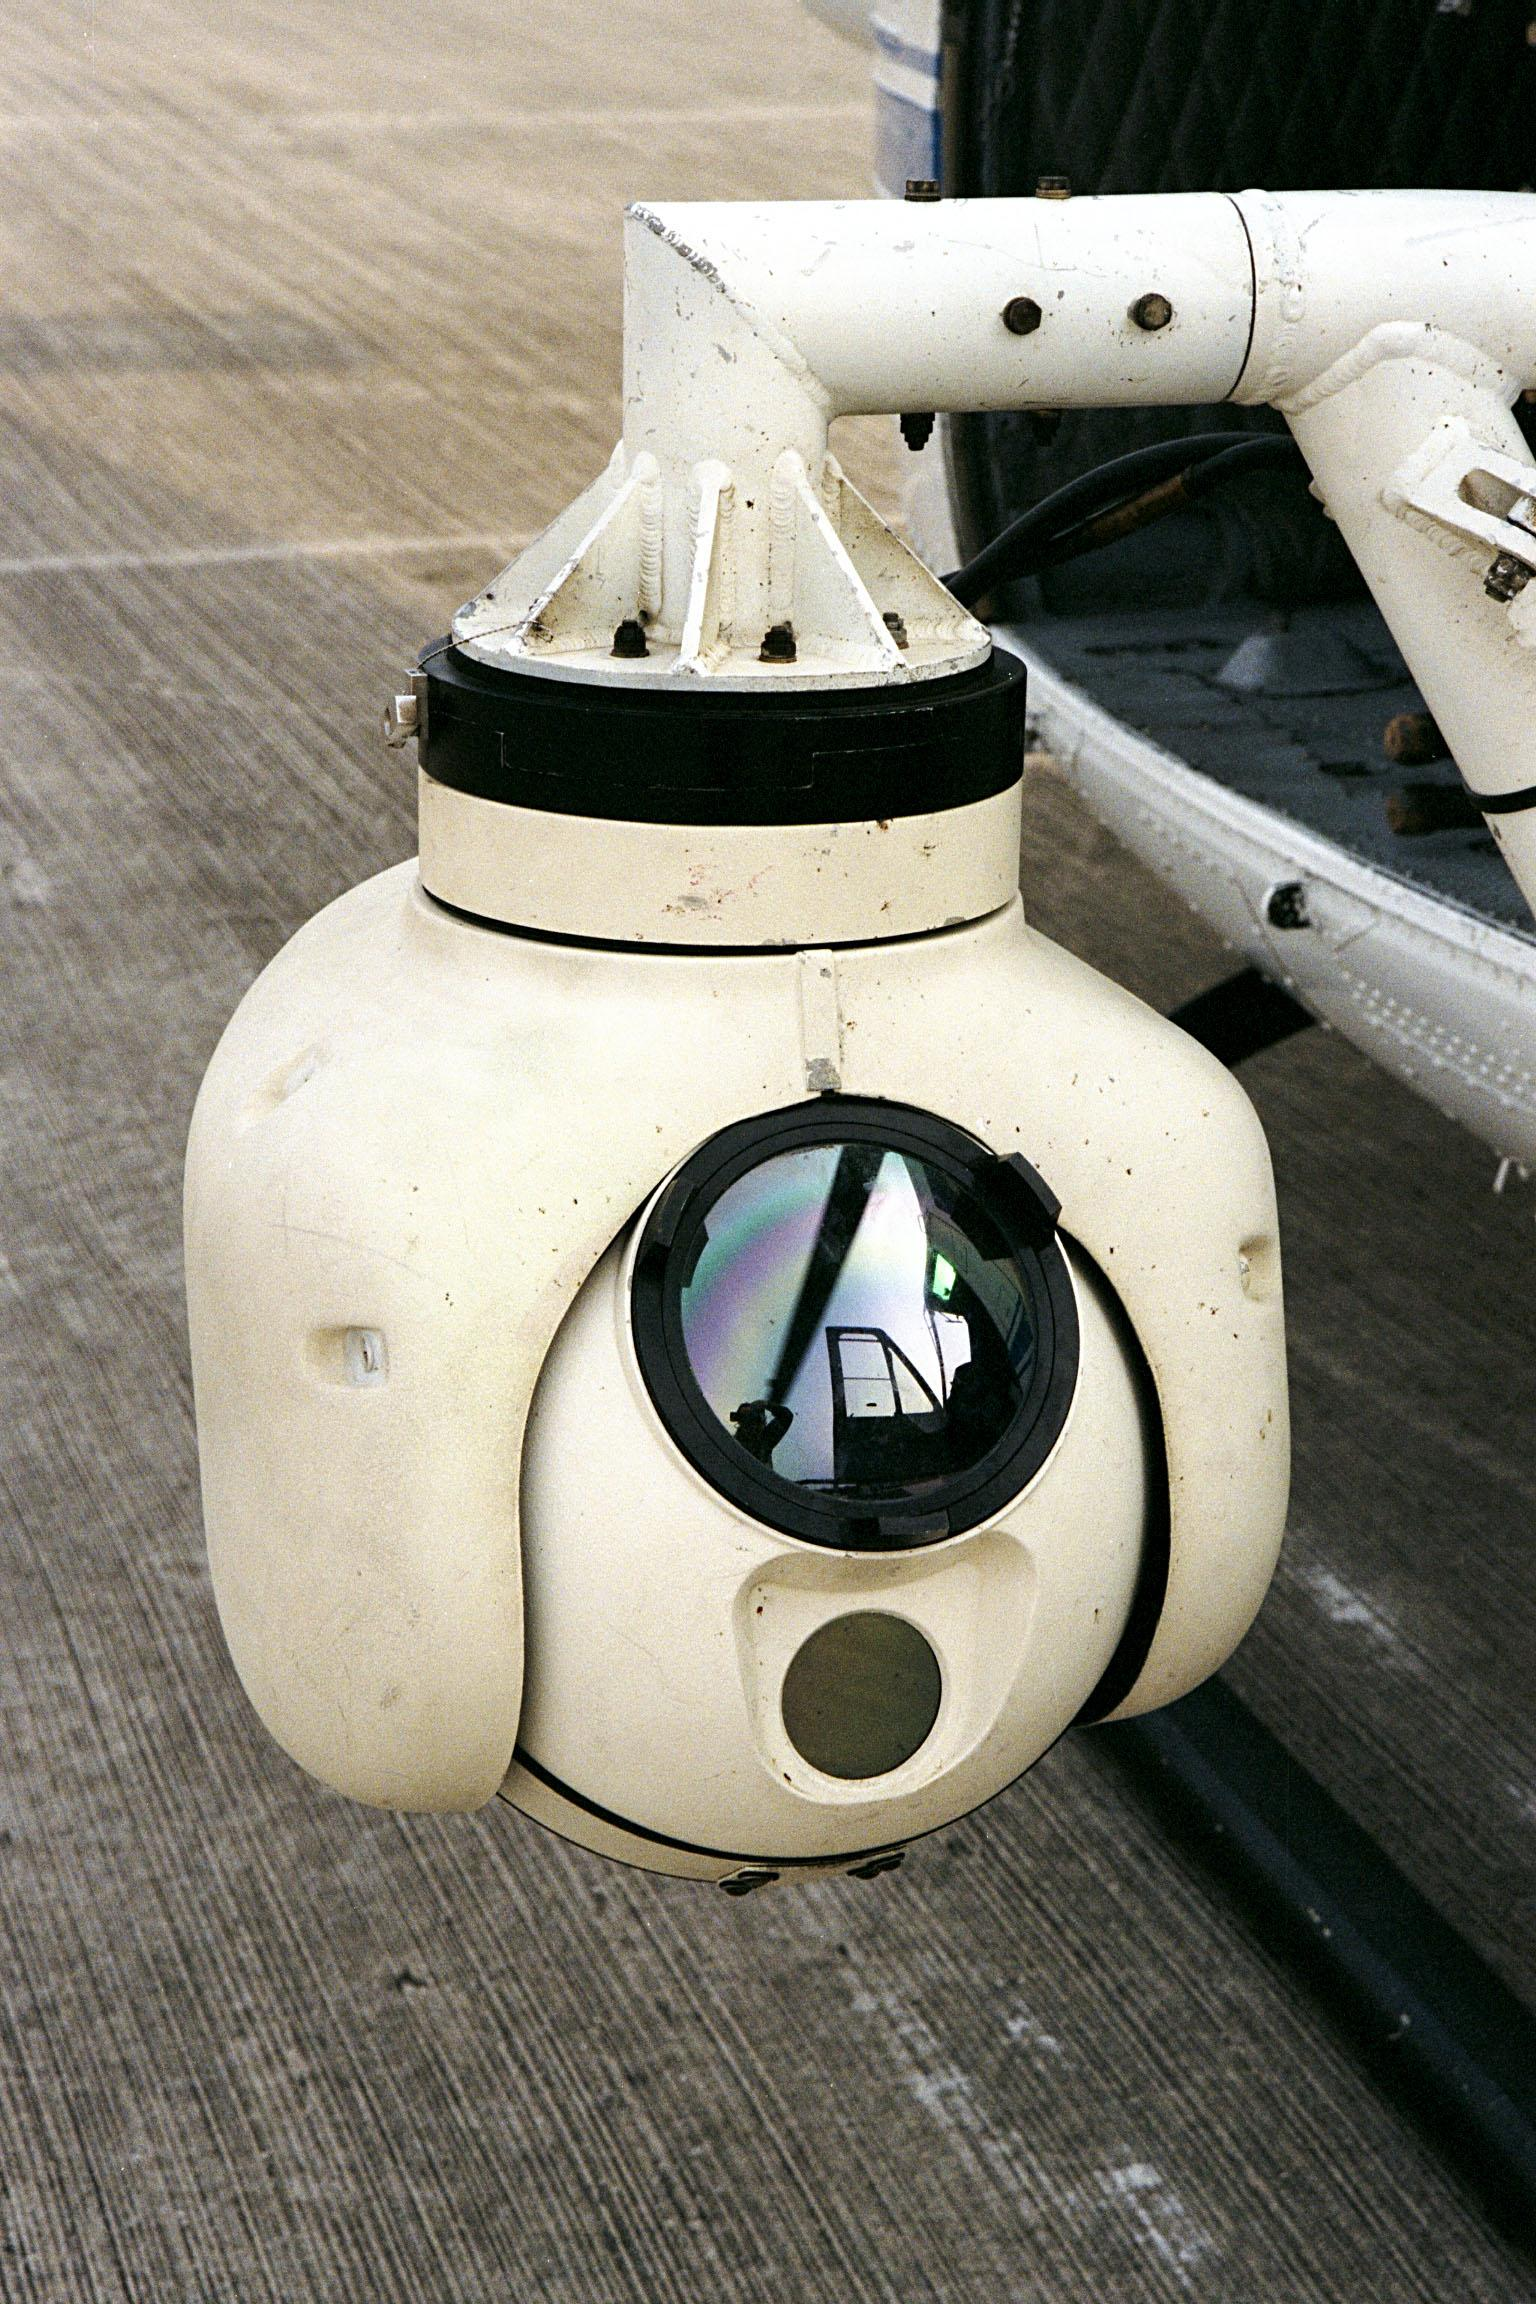
\includegraphics[height=0.5\textwidth]{Immagini/infrareduav}
 \caption{Una fotocamera ad infrarossi montata sul di un \ac{UAV}}
 \label{img:infrareduav}
\end{figure}

I sensori biologici sono sensori in grado di rilevare la presenza di microrganismi nell'aria e vari altri fattori biologici,
mentre i sensori chimici utilizzano spettroscopia laser per analizzare la concentrazione di ciascun elemento in aria.

\subsection*{Sorveglianza Aerea}
Grazie agli \ac{UAV} è possibile sorvegliare vaste aree a basso costo, questo tipo di operazioni comprende: mappatura degli incendi,
monitoraggio del bestiame, sicurezza domestica, stradale e pattugliamento anti-pirateria.
Molto importante è quest'ultimo aspetto, la sicurezza territoriale, delle frontiere e lotta ai narcotrafficanti, infatti nel 2011,
gli Stati Uniti hanno collaborato con il Messico per arginare il fenomeno dell'immigrazione clandestina e del traffico di sostanze 
stupefacenti attraverso il monitoraggio del loro confine

\subsection*{Indagini Geofisiche}
Gli \ac{UAV} sono impiegati anche in indagini geomagnetiche, dove il differenziale del campo magnetico terrestre è utilizzato
per calcolare la struttura della sottostante roccia magnetica, spesso ciò è utile per cercare di predire la posizione di
miniere minerarie e petrolifere.

\subsection*{Trasporto}
Una delle meno comuni funzioni degli \ac{UAV} è quella del trasporto merci. La maggior parte dei carichi utili sono contenuti in un 
vano di carico interno, i carichi esterni invece possono essere legati alla fusoliera o fissati alle ali, in questo caso però ne
risentirà l'aerodinamica, quindi sono spesso racchiusi in un guscio.

\subsection*{Ricerca Scientifica}
Gli \ac{UAV} sono gli unici in grado di penetrare in aree che possono essere troppo pericolose per le imbarcazioni pilotate.
Per esempio la \emph{NOAA} (National Oceanic and Atmospheric Administration), nel 2006 ha iniziato ad utilizzare gli \ac{UAV} come
cacciatori di uragani, questo tipo di aeromobili è in grado di volare all'interno dell'uragano per comunicare quasi in tempo 
reale dati come pressione barometrica standard e dati di temperatura, anche molto vicini alla superficie dell'acqua,
direttamente al National Hurricane Center in Florida. \\ 
Ulteriori applicazioni per aerei senza pilota possono essere quelli del produttore britannico UAVSI, che ha progettato una
variante degli \ac{UAV} particolarmente adatta a climi rigidi, come l'Antartide.

\subsection*{Attacchi Armati}
Gli MQ-1 Predator sono \ac{UAV} armati con missili \ac{HELLFIRE}, 
sempre più utilizzati dagli Stati Uniti come piattaforme per colpire bersagli a terra. I Predators armati sono stati utilizzati 
alla fine del 2001 da basi in Pakistan e Uzbekistan, per lo più volti ad assassinare persone di alto profilo 
(capi terroristi, \dots) in Afghanistan. Da allora, ci sono stati molti casi di attacchi di questo tipo che si svolgono 
in Afghanistan, Pakistan, Yemen e Somalia. Il vantaggio di utilizzare un veicolo senza pilota, 
piuttosto che un aereo con equipaggio, in questi casi è quello di evitare un imbarazzo diplomatico nel caso in cui l'aeromobile 
venisse abbattuto e venissero catturati i piloti, dal momento che i bombardamenti si svolgono in paesi ritenuti cordiali e 
senza il permesso ufficiale di quei paesi.

\subsection*{Ricerca e Salvataggio}
\label{sec:rs}
Un altro ruolo importante per gli \ac{UAV} è quello nelle operazioni di ricerca e soccorso, grazie ad essi, infatti, è possibile
raggiungere agevolmente zone colpite da disastri naturali o causati dall'uomo, per permettere ricognizioni in tempi rapidi. \\
Proprio su un aspetto di questo particolare uso si soffermerà questa tesi: in queste situazioni sarà proprio compito dell'\ac{UAV}
ripristinare le comunicazioni in modo da consentire agli operatori di soccorso di dialogare tra loro, ed eventualmente con 
le persone (civili) coinvolte nella crisi.
\\[1cm]
L'utilizzo degli \ac{UAV} considerato in questa tesi è stato quello del ripristino e gestione delle comunicazioni in aree colpite da crisi 
in cui è molto importante riuscire a mantenere le connessioni attive per facilitare le operazioni di soccorso a seguito di calamità 
naturali o da avvenimenti particolari (terremoti, esondazioni,incidenti stradali, \ldots).

\section{Classificazione}
Gli \ac{UAV}  in genere rientrano in \emph{sei} categorie a seconda della loro funzione, ultimamente però i ruoli svolti raccolgono più
di una sola funzione in un solo aeromobile:

\begin{description}
 \item[Target and decoy] Fanno da obiettivo aereo o terrestre simulando un aeromobile o un missile nemico.
 \item[Reconnaissance] Forniscono informazioni sul campo di battaglia.
 \item[Combat] Hanno la capacità di attaccare in missioni ad alto rischio.
 \item[Logistics] \ac{UAV} specificamente progettato per il carico e la gestione della logistica.
 \item[Research and development] Utilizzati per sviluppare ulteriormente le tecnologie \ac{UAV}.
 \item[Civil and Commercial UAVs] \ac{UAV} sviluppati principalmente per applicazioni civili e commerciali.
\end{description}

È possibile un altro tipo di classificazione in termini di altitudine/range:

\begin{description}
 \item[Handheld] (altitudine di circa 600 m), circa 2 km di range.
 \item[Close] (altitudine massima 1500 m), più di 10 km di range.
 \item[NATO type] (massima altitudine 3000 m) più di 50 km di range.
 \item[Tactical] (altitudine di circa 5500 m), circa 160 km di range.
 \item[MALE] (altitudine media, lunga durata) altitudine oltre 9000 m, più di 200 km di range. 
 \item[HALE] (elevata altitudine, lunga durata) altitudine oltre 9100 m, range indefinito.
 \item[HYPERSONIC] (alta velocità, supersonico (Mach 1–5) o ipersonico (Mach 5+)) altitudine di circa 15200 m (sub-orbitale) e range oltre 200 km.
\end{description}

\section{Eventi civili che hanno coinvolto UAV}
Come già detto nell'introduzione, il vantaggio che deriva dall'utilizzo degli \ac{UAV} è l'utilizzo nelle missioni 
\emph{dull, dirty and dangerous}, negli ultimi anni ci sono state varie occasioni che hanno coinvolto gli \ac{UAV}:
\begin{itemize}
 \item Un importante coinvolgimento non bellico degli \ac{UAV} è stato durante il terremoto del Tohoku del 2011. I velivoli americani 
 \emph{Global Hawk} hanno sorvolato la Centrale nucleare di Fukushima Dai-ichi, in Giappone, per poter addentrarsi nelle zone vietate per
 le forti radiazioni. Lo scopo principale è stato quello di controllare i reattori dopo le esplosioni causate dal forte sisma.
 \item In Italia un recente utilizzo degli \ac{UAV} è stato durante il recente terremoto in \emph{Emilia}, sono stati utilizzati alcuni 
 velivoli per controllare le aree inaccessibili a causa delle macerie.
\end{itemize}

%\input{Capitoli/propagazione}
\chapter{Standard di Telefonia Mobile \emph{LTE}}
\label{cap:lte}
\begin{figure}[h]

\includegraphics[scale=0.5]{Immagini/lte}
\centering 
\end{figure}

Il sistema \ac{LTE} è un esempio importante di tecnologia radiomobile di quarta generazione (\emph{4G}) in grado di offrire servizi 
a larga banda. Se l'attuale generazione di reti di telecomunicazione mobile è nota come 3G, \ac{LTE} è, impropriamente, commercializzato 
come \emph{4G} (Fig. \ref{img:lte4g}).

\begin{figure}
 \centering
 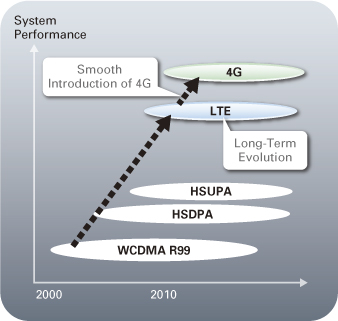
\includegraphics[scale=0.5]{Immagini/lte4g}
 \caption{L'evoluzione delle tecnologie mobili.}
 \label{img:lte4g}
\end{figure}

Secondo \ac{3GPP}, in \ac{LTE} sono identificati una serie di requisiti ad alto livello;
\begin{itemize}
 \item Riduzione dei costi per bit.
 \item Fornitura di più servizi a costi inferiori e con migliore esperienza utente.
 \item Flessibilità nell'utilizzo di bande frequenza nuove o esistenti.
 \item Architettura semplificata.
 \item Consentire un ragionevole consumo energetico del terminale.
\end{itemize}

Nonostante ci sia una sostanziale differenza rispetto ai suoi predecessori, \ac{LTE} è considerato un'evoluzione dello standard \emph{3G},
Nella tabella \ref{tab:confronto}, sono mostrate le principali differenze con le tecnologie precedenti:

 \begin{table}[h]\footnotesize
  \caption{Confronto tra le attuali e future tecnologie mobili}
  \label{tab:confronto}
  \begin{tabularx}{\textwidth}{XXXXXX}
    \toprule
      & WCDMA (UMTS) & HSDPA & HSDPA+ & LTE & LTE Advanced \\
    \midrule
      Max Downlink Speed & 384 kb/s & 14 Mb/s & 42 Mb/s & 326,4 Mb/s & 3,3 Gb/s \\
      Max Uplink Speed & 128 kb/s & 5,7 Mb/s & 11 Mb/s & 86,4 Mb/s & Sconosciuto \\
      Latency round trip time (ms) & 150 & 100 & 50 & ~ 10 & Sconosciuto \\
      3GPP Releases & Rel 99/4 & Rel 5/6 & Rel 7 & Rel 8 & Rel 10 \\
      Access methodology & CDMA & CDMA & CDMA & OFDMA / SC-FDMA & OFDMA Ibrido / SC-FDMA \\
    \bottomrule
    \end{tabularx}
  \end{table}

I motivi che hanno spinto a questa nuova tecnologia sono stati vari:
\begin{itemize}
 \item Necessità di garantire la continuità della competitività del sistema 3G per il futuro.
 \item Domanda degli utenti per velocità di trasferimento dati più elevate e qualità del servizio.
 \item Sistema ottimizzato di commutazione a pacchetto.
 \item Continua richiesta di riduzione dei costi (CAPEX e OPEX).
 \item Complessità bassa.
 \item Evitare un'inutile frammentazione delle tecnologie per la banda di funzionamento.
\end{itemize}

\section{Caratteristiche}
\label{sub:caratteristiche}
Lo standard \ac{LTE} affronta l'aggiornamento dal \emph{3G UMTS} verso quello che sarà chiamato standard comunicazione mobile di quarta 
generazione \emph{4G}. La maggior parte del lavoro mira a semplificare l'architettura del sistema, per esempio per le 
chiamate vocali, come discusso nel paragrafo \ref{sub:voice}, da una rete a commutazione a pacchetto (per i dati) e a commutazione a 
circuito (per le chiamate vocali) dell'attuale tecnologia \emph{UMTS}, verso un architettura completamente basata su \emph{IP}. \\
L'interfaccia fisica di trasmissione radio utilizzata in \ac{LTE} è detta \emph{E-UTRA}, le sue principali caratteristiche sono:
\begin{itemize}
 \item Velocità di download di picco di $299 Mbit/s$ e upload fino a $75.4 Mbit/s$.
 \item Latenze ridotte (inferiori ai 100 ms per il passaggio dallo stato idle allo stato active, ed in-
  feriori ai 5 ms per piccoli pacchetti IP)
 \item Migliorato il supporto per la mobilità, esemplificato da supporto per i terminali in movimento fino a $350 km/h$ o $500 km/h$ 
  a seconda della banda di frequenza.
 \item \emph{OFDMA} per il downlink\footnotemark[1] e \emph{SC-FDMA} per l'uplink\footnotemark[2].
 \item Supporto per i sistemi di comunicazione \ac{FDD} e \ac{TDD} e half-duplex \ac{FDD} con la stessa tecnologia di accesso radio.
 \item Supporto per dimensioni delle celle variabili: da decine di metri di raggio (femto e picocelle) fino a $100 km$ di raggio (macrocelle).
  Le bande di frequenza più basse sono utilizzate nelle zone rurali, con dimensioni cellulari da $5 km$ con prestazioni ottimali, fino a $100 
  km$ con prestazioni accettabili. Nelle aree urbane e urbane, bande di frequenza più elevate (ad esempio $2,6 GHz$ in EU) sono usate per 
  sostenere banda larga ad alta velocità mobile. In questo caso, le dimensioni delle celle può essere $1 km$ o anche meno.
 \item Supporto per almeno 200 clienti attivi per cella da $5 MHz$.
 \item Supporto per l'inter-operabilità e la coesistenza con tecnologie precedenti: gli utenti possono avviare una chiamata o il 
  trasferimento di dati in una zona con uno standard \ac{LTE}, e, se la copertura non è disponibile, continuare l'operazione senza alcuna 
  azione da parte loro passando a tecnologi precedenti come \emph{GSM / GPRS} o \emph{W-CDMA} o anche le reti \emph{UMTS}.
 \item Elevata efficienza spettale (numero di bit/s trasmessi per ogni Hz impiegato) 3 volte superiore alla più evoluta versione 
  dell'\emph{UMTS}, ovvero l'\emph{HSPA}.
\end{itemize}
\footnotetext[1]{Collegamento tra una stazione base e la stazione mobile ad essa associata}
\footnotetext[2]{Percorso dei dati da un telefono cellulare alla centrale}

 \subsection{Standard e frequenze}
 Nell'Unione Europea lo standard \ac{LTE} lavora sulle seguenti bande di frequenza:
 \begin{description}
  \item[800 MHz] in Italia dal 2013 sarà possibile sfruttare questa banda non appena sarà completo il passaggio al digitale terrestre
  \item[900 MHz] questa banda attualmente imegnata dal \emph{GSM} attraverso un \emph{refarming dello spettro} sarà disponibile per 
		  l'\ac{LTE}
  \item[1800 MHz] entro il 2012 saranno disponibili alcuni canali occupati dal GSM
  \item[2600 MHz] frequenze libere tranne che in alcune zone utilizzate dal ministero della difesa o da radar
 \end{description}
 
\subsubsection{OFDMA}
Uno degli elementi chiave di \ac{LTE} è l'uso di \ac{OFDM} per trasportare il segnale e gli schemi di accesso associati: \emph{OFDMA} 
(Orthogonal Frequency Division Multiple Access) e \emph{SC-FDMA} (Single Carrier Frequency Division Multiple Access). \\
\ac{OFDM} è già utilizzato in altri sistemi come \emph{WLAN} e \emph{WiMAX} per l'audio e il video \emph{broadcasting}; l'\ac{OFDM} ha
molti vantaggi tra cui la robustezza al \emph{fading} multiplo e alle interferenze.
\ac{OFDM} è un tipo di trasmissione che usa un gran numero di portanti vicini tra loro, modulati con basso \emph{symbol rate}. Normalmente 
ci si aspetterebbe che questi segnali interferiscano l'uno con l'altro, ma facendo in modo che siano ortogonali tra loro non c'è 
interferenza reciproca. Ciò si ottiene spaziando le portanti del reciproco del periodo di simbolo. \\
Questo significa che quando i segnali sono demodulati avranno un numero intero di cicli nel periodo di simbolo e il loro contributo si 
somma a zero, quindi non vi è alcun contributo di interferenza. 
I dati da trasmettere sono suddivisi su tutte le portanti, e attraverso l'utilizzo di tecniche di correzione di errore, se alcune 
frequenze portanti vengono perse a causa di effetti di \emph{fading} multiplo, i dati possono essere ricostruiti.  \\
Inoltre avendo dati trasmesso ad un basso \emph{symbol rate} attraverso tutte le portanti significa che gli effetti di riflessione e 
interferenza intersimbolica possono essere superati. Significa anche che reti a singola frequenza, in cui tutti i trasmettitori possono
trasmettere sul canale stesso, possono essere implementate.

\begin{figure}
 \centering
 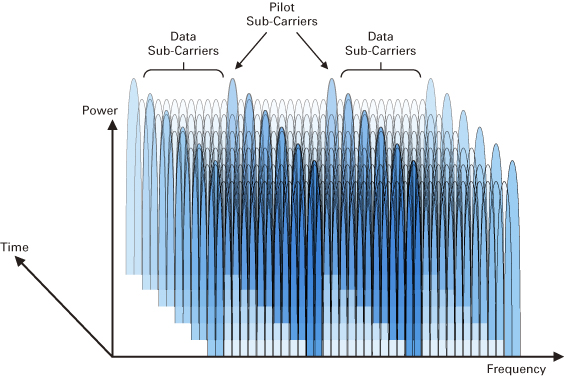
\includegraphics[scale=0.5]{Immagini/ofdma}
 \caption{OFDMA.}
 \label{img:ofdma}
\end{figure}
 
% \subsubsection{MIMO}
% L'acronimo \emph{MIMO} vuol dire \emph{Multiple-Input and Multiple-Output}, cioè entrate multiple ed uscite multiple, in \ac{LTE} sta ad 
% indicare la possibilità di un utilizzo di antenne multiple sia per il mittente per il ricevente per migliorare le prestazioni della
% comunicazione, come mostrato nella fiugra \ref{img:mimo}. \\
% La tecnologia \emph{MIMO} ha attirato l'attenzione nelle comunicazioni wireless, perché offre un aumento significativo del 
% \emph{throughput}, la capacità di trasmissione effettivamente utilizzata, senza ulteriore larghezza di banda o aumento di potenza di 
% trasmissione.
% Questi risultati possono essere raggiunti diffondendo la stessa potenza totale sulle antenne per ottenere una matrice di guadagno (Fig.
% \ref{img:mimomatrix} che migliora l'efficienza spettrale (più bit per secondo per hertz di banda) o per ottenere un guadagno che 
% migliora l'affidabilità collegamento (fading ridotto). 
% A causa di queste proprietà, \emph{MIMO} è una parte importante delle moderne tecnologie di comunicazione wireless come 
% \emph{IEEE 802.11n (Wi-Fi)}, \emph{4G}, \emph{WiMAX} e \emph{HSPA +}, oltre che, ovviamente, \ac{LTE}.
% 
% \begin{figure}[!h]
% 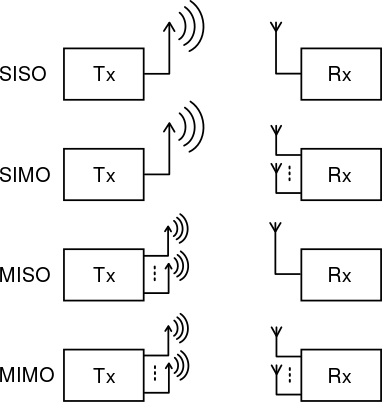
\includegraphics[scale=0.5]{Immagini/mimo}
% \centering 
% \caption{Configurazioni SISO, SIMO, MISO e MIMO, l'ingresso e l'uscita si riferiscono al canale radio che porta il segnale, non alle 
% antenne che hanno i dispositivi.}
% \label{img:mimo}
% \end{figure}
% 
% \begin{figure}[!h]
% 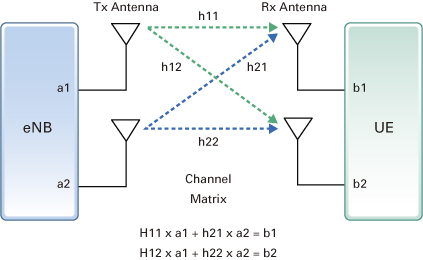
\includegraphics[scale=0.5]{Immagini/mimomatrix}
% \centering 
% \caption{Matrice di guadagno $2 \times 2$.}
% \label{img:mimomatrix}
% \end{figure}

 \subsection{Architettura di rete}
 La rete di accesso di \ac{LTE}, detta anche \ac{E-UTRA}, è costituita da un unico elemento, il cosiddetto \ac{eNB}.
 In \ac{LTE}, al contrario che nelle precedenti tecnologie, è possibile semplificare l'architettura di rete nel solo \ac{eNB} (Fig. \ref{img:enb}),
 in quanto tutti dati, anche quelli voce, viaggiano su protocolli a pacchetto; il grande vantaggio, inoltre, è che i nodi sono 
 interconnessi tramite interfacce standardizzate in modo da garantire la compatibilità con le tecnologie precedenti. \\
 Gli \ac{eNB} sono interconnessi tramite le interfacce \emph{X2}. Si presume che esista sempre un'interfaccia X2 tra gli 
 \ac{eNB} che devono comunicare tra loro, ad esempio, per il supporto del trasferimento dell'\ac{UE} nello stato \emph{active}. 
 Gli \ac{eNB} sono collegati anche mediante l'interfaccia \emph{S1} alla \emph{EPC} (Evolved Packet Core). L'interfaccia \emph{S1} 
 supporta una relazione molti-a-molti tra \emph{aGW} e \ac{eNB}.
 
 \begin{figure}[!h]
 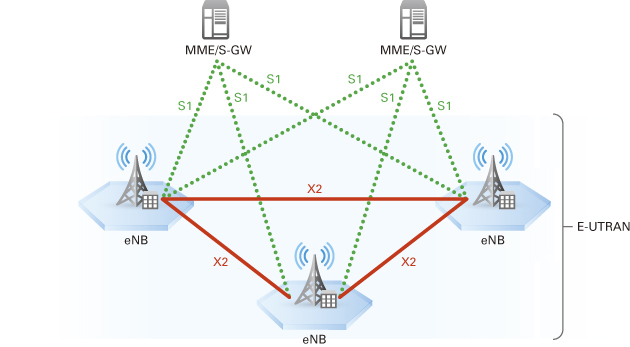
\includegraphics[scale=0.5]{Immagini/enb}
 \centering 
 \caption{Architettura di rete \ac{LTE}}
 \label{img:enb}
 \end{figure}
 
 \subsubsection{User Equipment}
 Il dispositivo \ac{LTE} è detto \ac{UE} come già avveniva con l'\emph{UMTS}, questo termine sta proprio ad evidenziare l'avanzato apparato
 tecnologico che si porta dietro l'utente. L'\ac{UE} è costituito da due parti: il \emph{Mobile Equipment}, cioè l'hardware che costituisce
 il dispositivo e il software ch permette la connessione alla rete, e la \emph{Universal Subscriber Identity Module}, il circuito integrato
 che contiene le informazioni legate all'utente, alla rete e ai servizi supportati.
  
\subsection{Quality of Service}
\label{sec:qos}
L'\ac{LTE} fornisce diverse qualità di servizio \ac{QoS}, ogni flusso informativo è associato ad una specifica classe di \ac{QoS}, i 
livelli di \ac{QoS} offerti sono due:
\begin{description}
 \item[GBR] (minimum Guaranteed Bit Rate): questo tipo di servizio offre risorse dedicate per tutta la durata della trasmissione, alti
 data rate, ritardi contenuti e  tassi d'errore contenuti;  l'utilizzo principale è quello voce, come le chiamate vocali o il \emph{VoIP}.
 \item[Non-GBR]: questo servizio sono utilizzati per applicazioni che non richiedono bitrate particolarmente elevati, come il web browsing
 o i trasferimenti FTP.
\end{description}

 \subsection{Mobilità e Handover}
 Un terminale all'interno di \ac{LTE} può trovarsi in tre stati: \emph{detached}, \emph{active}, \emph{idle}.
 \begin{figure}[!h]
 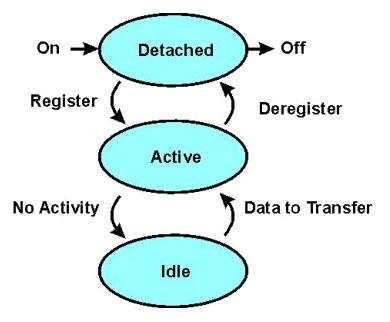
\includegraphics[scale=0.5]{Immagini/ltestatus}
 \centering 
 \caption{Stati di un dispositivo mobile \emph{LTE}.}
 \end{figure}
 Non appena il dispositivo viene acceso, esso si trova nello stato \emph{detached}: è attivo ma non è ancora connesso alla rete. Questa
 è la fase dell'instaurazione della connessione, l'utente è registrato presso l'eNB e passa nello stato \emph{active}. Infine, se l'utente
 non trasmette o riceve per un determinato tempo passa nello stato \emph{idle}. \\
 La posizione di un utente è nota alla rete attraverso la granularità di una \ac{TA}, l'\ac{UE} è memorizzato in un'area geografica, che
 potrebbe essere una \ac{TA} o un elenco di \ac{TA}; il nodo di controllo avvia il \emph{paging} per ciascun \ac{eNB} con celle 
 appartenenti all'\ac{UE}, l'utente passa da \emph{idle} a \emph{active} e può ricevere una chiamata. Ogni \ac{eNB} può contenere celle 
 appartenenti a diverse \ac{TA}, mentre ogni cella può appartenere ad una sola \ac{TA}. \\
 Con riferimento alla figura \ref{img:enb} in \ac{LTE} esistono due tipi di \emph{Handover}, essi si distinguono in base all'interfaccia su
 cui si muove l'\ac{UE}, \emph{X2} o \emph{S1}:
 \begin{description}
  \item[X2] Si riferisce al caso in cui l'utente si muove tra due \ac{eNB}, sempre gestiti dallo stesso \emph{aGW}, cioè all'interno della
  stessa \ac{TA}. L'\emph{handover} avviene sull'interfaccia \emph{X2} tra l'\ac{eNB} su cui è attualmente agganciato (\emph{serving)} e
  il prossimo \ac{eNB} che servirà l'\ac{UE} (\emph{target}), solo questi due nodi sono coinvolti, di conseguenza l'\emph{handover} è
  rapido e richiede poche risorse. Al termine della procedura l'\emph{aGW} è avvisato del cambio di posizione. \\
  Inoltre a seconda delle esigenze dell'\ac{UE} possono avvenire due tipi di \emph{handover}, i quali, ovviamente, sono strettamente legati
  al \ac{QoS} (paragrafo \ref{sec:qos}):
  \begin{itemize}
   \item seamless: questo tipo di \emph{handover} è particolarmente sensibile ai ritardi, quindi è utilizzato nel caso in cui l'\ac{UE} 
   abbia bisogno di servizi \emph{real-time} come, ad esempio, una chiamata vocale.
   \item lossless: in questo tipo di \emph{handover}, invece, lo scopo principale è mantenere un basso tasso di errori e ridurre le perdite
   di pacchetti.
  \end{itemize}

  \item[S1] In questo caso l'\ac{UE} si muove da una \ac{TA} ad un'altra. Questo tipo di \emph{handover} in \ac{LTE} è di tipo \emph{hard},
  la connessione è brevemente interrotta durante il passaggio da un \ac{eNB} ad un altro, il motivo principale di questa interruzione è
  l'assenza di un nodo di controllo che gestisca il traffico di segnalazione. Di conseguenza la rete è semplificata ad esempio rispetto a
  quella \emph{UMTS}.
 \end{description}

 
 
 \subsection{Chiamate vocali}
 \label{sub:voice}
Lo standard \ac{LTE} supporta solo la \emph{commutazione a pacchetto} nelle sue reti IP. Le chiamate vocali nel \emph{GSM}, \emph{UMTS} e 
\emph{CDMA} sono a circuito, quindi con l'adozione dell'\ac{LTE}, gli operatori telefonici dovrebbero riprogettare la loro rete voce. \\
La differenza principale tra commutazione a pacchetto ed a circuito è che nella prima il flusso di informazione è segmentato in 
\emph{pacchetti} di lunghezza limitata o fissa, come avviene in internet con IP; al contrario, la commutazione a circuito, prevede il 
frazionamento della capacità trasmissiva totale per ogni utente. \\
Per ovviare alla riprogettazione della rete sono state proposte tre soluzioni:
\begin{description}
 \item[VoLTE] (Voice Over \ac{LTE}) Questo tipo di approccio prevede di consegnare la voce come se fosse un flusso all'interno del 
 trasporto dati di \ac{LTE}, in questo modo si aggira la commutazione a pacchetto continuando ad utilizzare quella a circuito.
 \item[CSFB] (Circuit Switched FallBack) In questo approccio, \ac{LTE} fornisce il servizio dati e, quando richiesto il servizio voce, 
 automaticamente ricade nella commutazione a circuito.
 \item[SVLTE] (Simultaneous Voice and \ac{LTE}) Questo approccio, invece, fa coesistere le due tecnologie, adottando l'utilizzo della 
 commutazione a pacchetto per la connessione dati e della commutazione a circuito per le chiamate vocali. 
\end{description}
Un altro tipo di approccio prevederebbe di utilizzare la connessione dati anche per le chiamate voci, come accade per \emph{Google Talk} o
\emph{Skype}, ma è troppo complesso perché costringerebbe ogni utente ad avere una connessione attiva sul proprio dispositivo. \\
La maggior parte dei sostenitori principali di \ac{LTE} hanno preferito e promosso \emph{VoLTE} fin dall'inizio, anche se la soluzione 
migliore sarebbe di passare alla commutazione a pacchetto.
Nei paesi dove questa tecnologia è stata già adottata, nell'attesa della standardizzazione del \emph{VoLTE}, a causa dell'elevata
domanda per le chiamate vocali, è stato necessario introdurre \emph{CSFB} come misura provvisoria. Quindi quando si effettua o si riceve
una chiamata vocale, i telefoni \ac{LTE} ricadranno sulla vecchie reti \emph{2G} e \emph{3G} per la durata della chiamata. \\

\ac{LTE} supporta inoltre le chiamate vocali ad alta qualità (\emph{Voice HD}), per garantire la compatibilità, \ac{3GPP} richiede il codec
\emph{AMR} a banda stretta, ma il codec consigliato per il \emph{VoLTE} è a banda larga, inoltre, nelle reti \ac{3GPP} è obbligatorio il 
campionamento a $16 KHz$. Questo tipo di tecnologia, però, richede che sia il mittente che il destinatario la supportino.


\section{LTE in Italia}
In Italia, il 30 settembre 2011 si è conclusa l'asta per la concessione delle frequenze 4G \ac{LTE} delle tre frequenze disponibili: 
$800$, $1800$ e $2600 Mhz$. Il \date{27 Giugno 2011} nella Gazzetta Ufficiale viene pubblicato il bando per l'assegnazione delle 
frequenze agli operatori mobili italiani:
\begin{itemize}
 \item banda $800 MHz$: \emph{``fino a 6 lotti di frequenze FDD, ciascuno di ampiezza pari a 5 MHz in spettro accoppiato, assegnabili su base 
 nazionale, nominati da 1 a 6.''} \\
 Di questi sei lotti ne sono stati acquistati due per ognuna di queste compagine: \emph{Vodafone Italia}, 
 \emph{Telecom Italia} e \emph{Wind Telecomunicazioni}.
 \item banda $1800 MHz$: \emph{``fino a 3 lotti di frequenze FDD, ciascuno di ampiezza pari a 5 MHz in spettro accoppiato, assegnabili su base 
 nazionale, nominati da 1 a 3.''} \\
 Un blocco a testa è stato aggiudicato da \emph{Vodafone Italia}, \emph{Telecom Italia} e \emph{3 Italia}.
 \item banda $2000 MHz$: \emph{``1 lotto di frequenze TDD di ampiezza pari a 15 MHz, assegnabile su base nazionale, nominato lotto A.''} \\
 Per questo  lotto non è stata effettuata nessuna offerta.
 \item banda $2600 MHz$: \emph{``fino a 12 lotti di frequenze FDD, ciascuno di ampiezza pari a 5 MHz, in spettro accoppiato, assegnabili su base 
 nazionale, nominati da 3 a 14, e 2 lotti di frequenze TDD, ciascuno di ampiezza pari a 15 MHz, assegnabili su base nazionale, nominati 
 lotto B e C, con esclusione delle frequenze 2500-2510 MHz e 2620-2630 MHz nei lotti FDD e delle frequenze 2600-2620 MHz nei lotti TDD.''} \\
 \emph{3 Italia} e \emph{Wind Telecomunicazioni} si aggiudicano quattro blocchi, tre \emph{Vodafone Italia} e \emph{Telecom Italia}.
\end{itemize}

% \section{Sviluppi futuri: LTE-Advanced}
%  L'obiettivo di \ac{3GPP} \ac{LTE} Advanced è quello di raggiungere e superare i requisiti \emph{ITU} (International Telecommunication 
%  Union). \ac{LTE} Advanced dovrebbe essere compatibile e condividere le stesse frequenze dell'attuale \ac{LTE}. \\
%  Uno dei più grandi vantaggi di \ac{LTE} Advanced sarà la capacità di sfruttare avanzate reti topologiche: reti eterogenee ottimizzate con 
%  un mix di macrocelle con nodi a bassa potenza come picocelle e femtocelle. \\
%  \ac{LTE} Advanced introduce anche una multiportante per essere in grado di utilizzare una ultra banda larga, fino a $100 MHz$ di spettro 
%  supportando velocità molto elevate. Nella fase di ricerca che ha portato ad \ac{LTE} Advanced le proposte sono state svariate, esse 
%  possono essere suddivise principalmente in:
%  \begin{itemize}
%   \item Trasmissione e ricezione coordinata (\emph{CoMP}).
%   \item Supporto per il \emph{SU-MIMO} sull'antenna trasmittente dell'\ac{UE}.
%   \item Banda del sistema scalabile superiore a 20 MHz, fino a 100 MHz.
%   \item Flessibilità dello spettro.
%   \item Cognitive radio
%   \item Configurazione e funzionamento di rete automatico e autonomo.
%   \item Maggiore precodifica e rilevazione e successiva correzione degli errori.
%   \item Gestione dell'interferenza e la soppressione.
%   \item Assegnazione della larghezza di banda asimmetrica per ac{FDD}.
%   \item Uplink ibrido con \emph{OFDMA} e \emph{SC-FDMA}.
%   \item Accesso multiplo delle portanti allo spettro.
%  \end{itemize}
  

\chapter{Analisi di Copertura della Rete}
\label{cap:analisi}
Il simulatore ha permesso di ottenere i risultati riguardo la copertura dell'apparato \ac{LTE},
  
\section{Modellazione dello scenario}
\label{cap:dem}
In questa tesi è stato possibile simulare un modello tridimensionale degli ostacoli relativo ad una mappa esistente utilizzando 
la rappresentazione digitale delle quote di un territorio, usufruendo delle cosiddette mappe \ac{DTM}.
Sopra questo base è stato applicato un modello degli ostacoli, per generare uno scenario \emph{simile} a quello reale.
   
\subsection{Area di simulazione}
\label{sec:areasimu}
Per ottenere i dati relativi all'elevazione di una determinata area è stato necessario suddividere l'area come fosse una griglia, ogni
elemento della griglia è detto \emph{pixel}, in questa tesi ogni pixel ha le dimensioni di un quadrato di lato 5 m. \\
Successivamente è stato necessario assegnare ad ogni pixel la latitudine e la longitudine associata al centro di esso, ogni coordinata
dista quindi dalle adiacenti di circa 5 m.
L'area presa in considerazione è di circa $1 km \times 1 km$, quindi con una semplice divisione si ottiene che l'area, suddivisa in pixel, 
presa in esame equivale ad una matrice formata da $200 \times 200$ elementi, di cui ogni elemento contiene le coordinate esatte del centro 
del pixel. \\
È stato quindi sviluppato un semplice programma in \emph{Java} che permette la stampa su file di questi quarantamila elementi della 
matrice, elencati in colonna.

\subsection{Modello del terreno DTM}
Attraverso l'utilizzo del sito \url{http://www.gpsvisualizer.com/} è stato possibile importare la matrice output del programma citato 
nel paragrafo \ref{sec:areasimu} per ottenere l'elevazione di ogni coordinata.
Le elevazioni elencate nel file di output sono state rielaborate in una matrice con un altro programma in \emph{Java}, il risultato è 
quindi una matrice $200 \times 200$ contenente i dati dell'elevazione per ogni coordinata.
In Matlab è possibile effettuare un plot della matrice per rappresentare in tre dimensioni il modello del terreno come mostrato nella 
figura \ref{img:codem}.
\begin{figure}[h]
\centering
\caption{Modello tridimensionale del terreno della zona tra Colle Oppio e la stazione Roma Termini}
\label{img:codem}
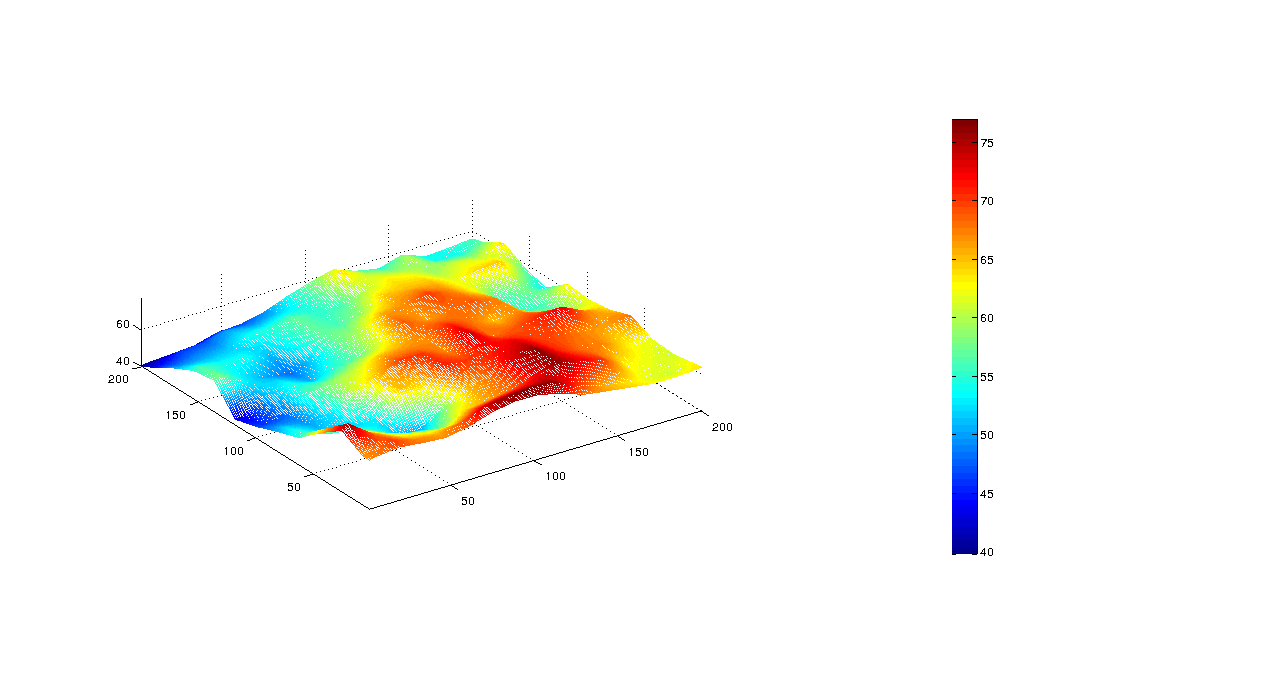
\includegraphics[scale=0.4]{Immagini/colleoppiodem}
\end{figure}

\subsection{Modello degli ostacoli}
Il processo che ha portato ad alla modellazione degli ostacoli è formato da più passi:
\begin{itemize}
\item Usufruendo delle \emph{API} di Google Maps è possibile fare una query http per ottenere la mappa dell'area interessata, in 
particolare per quanto riguarda l'area della zona tra Colle Oppio e la stazione Roma Termini è stato utilizzato l'url \\
\url{http://maps.google.com/maps/api/staticmap?center=41.895805,12.499113&zoom=15&size=1000x1000&sensor=false}
\begin{description}
\item \url{center=41.895805,12.499113} \\ indica le coordinate del centro della mappa statica.
\item \url{zoom=15} \\ indica il livello di zoom.
\item \url{size=1000x1000} \\ rappresenta la risoluzione dell'immagine.
\item \url{sensor=false} \\ in alcune applicazioni potrebbe essere necessario il sensore GPS per ottenere la posizione dell'utente, 
ma non è questo il caso
\item \url{&style=feature:all|element:labels|visibility:off} \\ infine aggiungendo questa stringa  al termine dell'url è possibile
togliere le etichette per visualizzare esclusivamente l'immagine della mappa.
\end{description}
il risultato è rappresentato nell'immagine successiva (\ref{img:comap}).
\begin{figure}[h]
\centering
\caption{Immagine statica della zona tra Colle Oppio e la stazione Roma Termini ottenuta tramite query http con Google Maps API.}
\label{img:comap}
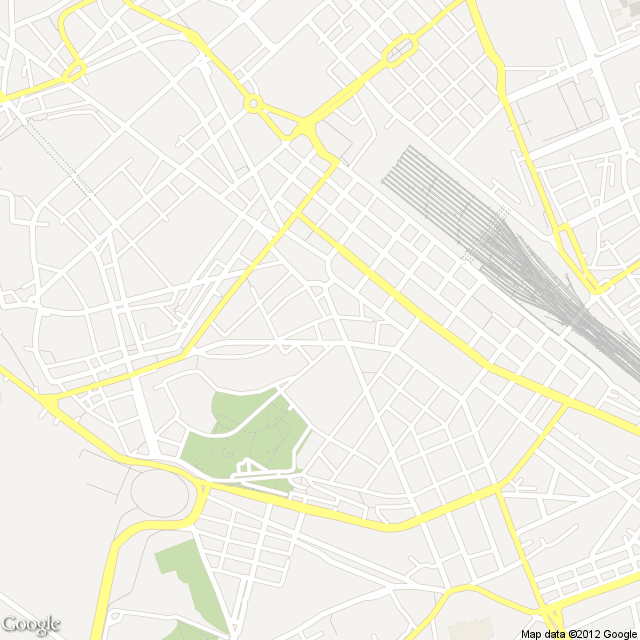
\includegraphics[scale=0.4]{Immagini/colleoppiomap}
\end{figure}
\item Il passo successivo è stato quello di rielaborare l'immagine per ottenere una maschera contenente gli ostacoli.
Per tale scopo è stato utilizzato \ac{GIMP}, software libero per la creazione e modifica di immagini digitali. \\
Per prima cosa è stata desaturata l'immagine, poi con l'aiuto di Google Earth è stato possibile evidenziare le aree piane e gli ostacoli;
è molto importante distinguere le due zone perché secondo i calcoli svolti in questa tesi, l'utente non può posizionarsi in 
corrispondenza degli ostacoli.
Avere quindi un modello degli ostacoli permette di verificare la copertura del sistema \ac{LTE} dell'\ac{UAV} in base alla posizione 
dell'utente. \\
Sono stati considerati come ostacoli costruzioni, monumenti e palazzi, quindi parchi, strade o, come in questo caso, la stazione in cui 
l'utente può sostare.
Gli ostacoli sono stati evidenziati in nero, tutto il resto è in bianco.
\begin{figure}[h]
\centering
\caption{Maschera degli ostacoli della zona tra Colle Oppio e la stazione Roma Termini ottenuta con \ac{GIMP} dalla mappa statica.}
\label{img:comask}

\includegraphics[scale=1]{Immagini/colleoppiomask}
\end{figure}

\subsection{Modello della mappa}
L'ultimo passo per arrivare ad un modello completo della mappa è stato quello di unire i due passaggi descritti nei due paragrafi
precedenti.
Il modello del terreno e la maschera degli ostacoli sono stati importati in Matlab, il risultato è quindi un modello tridimensionale
della mappa sul quale è applicata una maschera rappresentante la posizione di ogni ostacolo. \\
In Matlab è stato possibile sfruttare questo modello per ottenere una fedele rappresentazione tridimensionale dello scenario scelto. 
Sono stati utilizzati i dati dei modelli tridimensionali di \emph{Google Earth} come altezza, larghezza e lunghezza degli ostacoli, poi 
con l'aiuto di Matlab si è cercato di utilizzare questi dati per generare ostacoli con altezza, larghezza e lunghezza variabili nel
\emph{range} ottenuto da \emph{Google Earth}. \\
Il risultato è rappresentato nell'immagine sottostante. \\
\begin{figure}[!h]
\centering
\caption{Modello tridimensionale della zona tra Colle Oppio e la stazione Roma Termini.}
\label{img:modello}
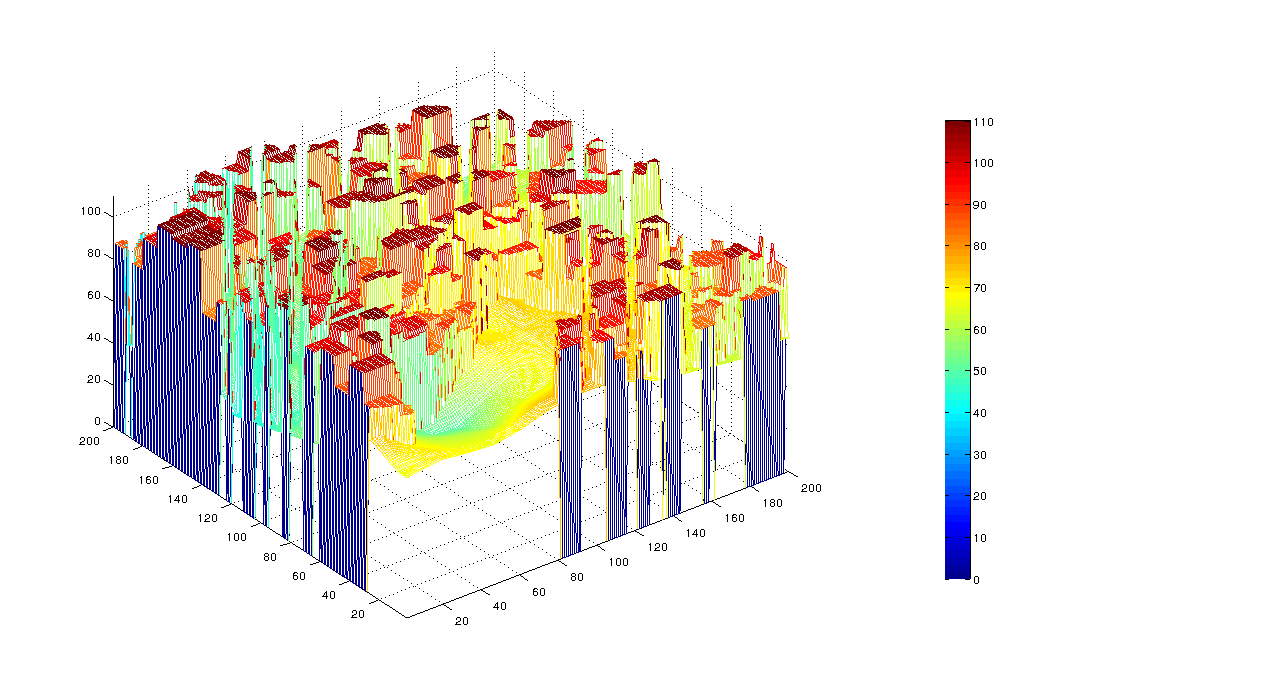
\includegraphics[scale=0.4]{Immagini/colleoppio}
\end{figure}
A questo punto è possibile utilizzare queste informazioni per modellare la copertura dell'apparato \ac{LTE} dell'\ac{UAV} su questo tipo 
di scenario.
\end{itemize}
\newpage
\section{Calcolo attenuazione}
Prima di descrivere come è stata calcolata l'attenuazione pixel $\times$ pixel è necessario richiamare alcuni concetti di propagazione
dell'onda elettromagnetica.

\subsection{Propagazione nello spazio libero}
Per propagazione nello spazio libero si intende una trasmissione del segnale elettromagnetico attraverso lo spazio libero o in mezzi 
tenui come l'atmosfera, in generale essa può suddividersi in radiopropagazione in un canale radio tra punti fissi (ponte radio) e 
radiopropagazione in un canale radiomobile tra terminali mobili e le stazioni radiobase. \\

\subsubsection{Attenuazione}
Un aspetto fondamentale di questo tipo di propagazione è l'attenuazione, questa può essere di due tipi:
\begin{description}
\item[attenuazione isotropica] è tipica dello spazio libero e la potenza diminuisce come $\frac{1}{d^{2}}$: \\
\[
p(d)=\frac{P_{T}}{4 \pi d^{2}}
\]
\item[attenuazione supplementare] si aggiunge a quella isotropica se il mezzo è diverso da quello vuoto.
\end{description}

\subsubsection{Fading} 
Nei collegamenti via etere all'ingresso del ricevitore il segnale giunge con improvvise e casuali variazioni di breve durata sia in 
ampiezza che in fase. Tali fluttuazioni sono note come fading o evanescenza. Il fenomeno è dovuto a varie cause.
Il \emph{fading per attenuazione} è dovuto alle variazioni fisiche dell'atmosfera che producono diverse attenuazioni del segnale in 
funzione della frequenza.
Il \emph{fading per interferenza} è dovuto all'interferenza tra i diversi segnali che partendo dal trasmettitore seguono molteplici 
percorsi prima di giungere al ricevitore. I segnali ricevuti hanno ampiezze e fase continuamente variabili poiché dipendono dallo 
stato fisico dell'atmosfera (pioggia, temporali, \ldots) dalla natura del suolo (mare, monti, \ldots) e dal cammino che le onde
elettromagnetiche seguono (onde dirette, onde riflesse dal suolo, \ldots).
I ricevitori sono dotati di opportuni sistemi di regolazione automatica atti a compensare ma non eliminare il fenomeno di fading.

\subsubsection{Diffrazione}
Il fenomeno della diffrazione permette la propagazione dei segnali radio sulla
superficie curva della Terra, oltre l'orizzonte e oltre 
i vari ostacoli che può incontrare. Anche nel caso in cui la potenza del segnale ricevuto decresce rapidamente quando il trasmettitore 
si muove all'interno di regioni così dette in ombra, il segnale generato dalla diffrazione è sufficientemente potente da produrre un 
segnale utile. \\
La diffrazione può essere spiegata mediante il principio di Huygen, che afferma che tutti i punti appartenenti ad un fronte d'onda 
possono essere considerati come sorgenti di nuove onde; tali onde si combinano per produrre un
nuovo fronte che si propaga nella 
stessa direzione del primo; è questo secondo
fronte d’onda che permette la propagazione del segnale nelle regioni in ombra. \\

\subsubsection*{Zone di Fresnel}
Mediante le zone di Fresnel è possibile caratterizzare l'attenuazione dovuta a diffrazione in relazione alla differenza di cammino 
che le onde
devono compiere per aggirare un ostacolo posto tra trasmettitore e ricevitore.
Le zone di Fresnel rappresentano regioni successive in cui le onde secondarie
devono percorrere, per raggiungere il ricevitore 
dal trasmettitore, una distanza
maggiore di $n\frac{\lambda}{2}$ rispetto al cammino lungo la \ac{LOS}.
\begin{figure}[h]
\centering
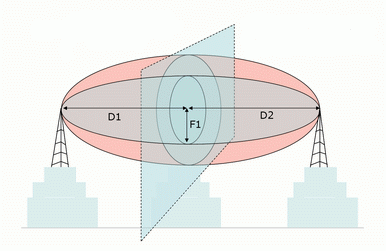
\includegraphics[height=0.5\textwidth]{Immagini/fresnel}
\caption{I confini delle zone di Fresnel costituiti da cerchi concentrici nel caso in cui tra le due antenne non sono presenti ostacoli.}
\label{img:fresnel}
\end{figure}
La differenza tra il cammino diretto e il cammino rifratto che attraversa ogni cerchio è $n\frac{\lambda}{2}$, i raggi dei cerchi che 
delimitano le zone di Fresnel dipendono dal punto in cui è posto il piano, così le zone avranno raggio massimo nel punto centrale tra 
i due dispositivi e tali raggi andranno a rimpicciolirsi se il piano è mosso tra trasmettitore e ricevitore. \\

\subsubsection*{Ostacolo singolo: modello a lama di coltello}
La stima dell’attenuazione del segnale causato da diffrazione per onde radio in un ambiente non ottimale, in presenza per esempio di 
costruzioni o colline, come modellato in questa tesi, è solitamente difficile da effettuare con precisione. Quando la zona d'ombra in 
cui si viene a trovare il dispositivo ricevitore è generata da un unico oggetto che si frappone tra ricevitore e trasmettitore, 
l'attenuazione causata dalla diffrazione può essere stimata considerando l'ostacolo come un piano il cui spessore è minimo. \\
Questo è il più semplice modello di diffrazione in cui l'attenuazione del segnale causata da un tale fenomeno viene messa in relazione 
con quanto l'ostacolo invade la prima zona di Fresnel: più l'ostacolo entra nella prima zona di Fresnel e più il segnale arriva al 
ricevitore attenuato. \\
Il campo elettrico ricevuto ha una precisa soluzione analitica:
\begin{align}
\mathbf{E}_{d} = \mathbf{E}_{0} I(v) = \mathbf{E}_{0} \frac{1+j}{2} \int_{2}^{\infty} e^{-j \frac{2 \pi}{2} t^{2}}\, dt
\label{eq:ed}
\end{align}
dove $\mathbf{E}_{d}$ è il campo elettrico ricevuto, $\mathbf{E}_{0}$ è il campo elettrico che si avrebbe nello spazio libero e $v$ è
il \emph{parametro di diffrazione di Fresnel-Kirkhoff}, pari a:
\begin{align*}
 \label{eq:parametrodiffrazione}
 v = h \sqrt{\frac{2(d_{1} + d_{2})}{\lambda d_{1} d_{2}}}
\end{align*}
dove
\begin{description}
\item $h$ è la distanza tra la congiungente tre le antenne e l'estremità dell'ostacolo, la distanza $h'$ nella figura \ref{img:knifeedge}
è detta \emph{franco}.
\item $d_{1}$, $d_{2}$ sono, rispettivamente, le distanze tra trasmettitore ed ostacolo e tra ostacolo e ricevitore.
\item $\lambda$ è la lunghezza d'onda, $\lambda = \frac{c}{f}$
\end{description}
\begin{figure}[!h]
\centering
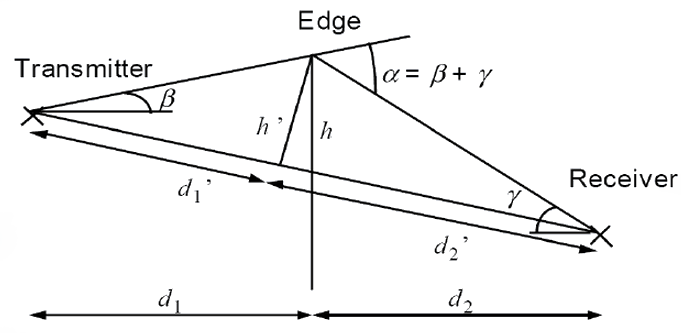
\includegraphics[height=0.5\textwidth]{Immagini/knifeedge}
\caption{Nell'origine l'ostacolo a lama di coltello con altezza h.}
\label{img:knifeedge}
\end{figure}
La funzione del parametro di diffrazione nell'equazione \ref{eq:ed} è l'integrale complesso di \emph{Fresnel}:
\begin{align}
\label{eq:integralefresnel}
I(v) = C(v) - jS(v)
\end{align}
con
\begin{align*}
 C(v)=\int_{0}^{v} \cos(\frac{\pi}{2}u^{2})\, du \\
 S(v)=\int_{0}^{v} \sin(\frac{\pi}{2}u^{2})\, du \\
\end{align*}
Le funzioni $C(v)$ e $S(v)$ sono dette, rispettivamente, integralcoseno e integralseno, il loro andamento, uno in funzione dell'altro,
è rappresentato nella figura \ref{img:cornu}, nella cosiddetta spirale di \emph{Cornu}:
\begin{figure}[!h]
\centering
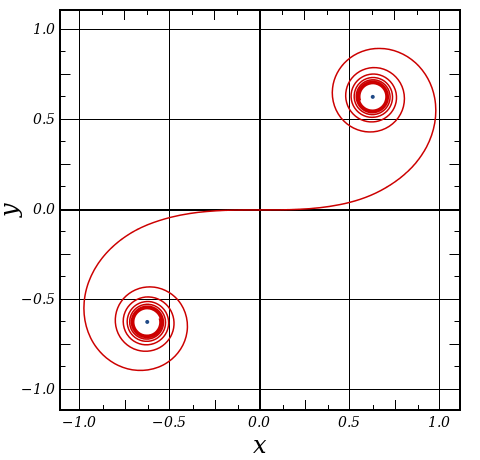
\includegraphics[height=0.5\textwidth]{Immagini/cornu}
\caption{Spirale di Cornu.}
\label{img:cornu}
\end{figure}
Dai valori asintotici $C(\infty) = S(\infty) = 0.5$ e $C(-\infty) = S(-\infty) = -0.5$, si ottiene, sostituendo nella (\ref{eq:ed}):
\[
\mathbf{E}_{d} = \mathbf{E}_{0} \frac{1+j}{2} 
\left \{ \left [ \frac{1}{2} - C(v) \right ] + j \left [ \frac{1}{2} - S(v) \right ] \right \}
\]
dalla quale si ottiene la \emph{perdita supplementare per diffrazione}:
\[
 L_{D}(dB) = -20 \log{F_{D}}
\]
Si definisce fattore di diffrazione, $F_{d}$, il rapporto tra l'ampiezza del campo ricevuto e quella nello spazio libero:
\begin{align*}
F_{d} \doteq& \left| \frac{\mathbf{E}_{d}}{\mathbf{E}_{0}}  \right| = \\
=& \frac{\sqrt{2}}{2} \left| \frac{1}{2} (1-j) - I(v) \right| = \\
=& \frac{\sqrt{2}}{2} \sqrt{ \left [ \frac{1}{2} - C(v) \right ]^{2} + \left [ \frac{1}{2} - S(v) \right ]^{2} }
\end{align*}
Nella figura \ref{img:fd} è rappresentato l'andamento di $F_{d}$ in funzione del parametro di diffrazione $v$. \\
\begin{figure}[!h]
\centering
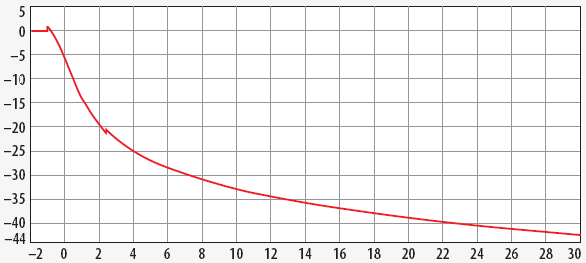
\includegraphics[height=0.5\textwidth]{Immagini/pathloss}
\caption{Andamento del fattore di diffrazione in funzione del parametro di diffrazione.}
\label{img:fd}
\end{figure}
Visivamente l'attenuazione per ostacolo singolo è ben descritta nella figura \ref{img:knifeedgeeffect}, il segnale trasmesso incide 
l'ostacolo, il quale diventa poi nuova sorgente e permette il passaggio del segnale al ricevitore, l'altezza dell'ostacolo può anche 
essere superiore a quella dell'apparato trasmittente o ricevitore.
\begin{figure}[!h]
\centering
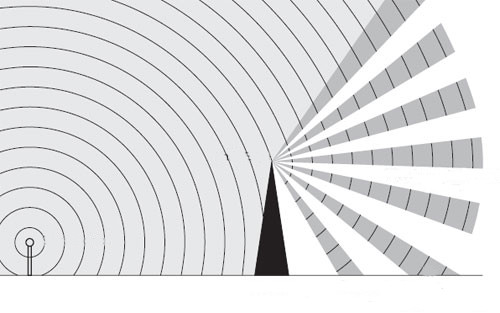
\includegraphics[height=0.5\textwidth]{Immagini/knifeedgeeffect}
\caption{Il segnale si propaga fino all'ostacolo che poi diventa la nuova sorgente.}
\label{img:knifeedgeeffect}
\end{figure}

\subsubsection*{Ostacolo multiplo: Metodo di Epstein-Peterson}
\label{sec:epsteinpeterson}
Nel caso di più ostacoli che si interpongono tra trasmettitore e ricevitore, è spesso utilizzato il modello di Epstein-Peterson.
Secondo questo modello la distanza tra trasmettitore e ricevitore può essere suddivisa in parti differenti, come mostrato in figura
\ref{img:epsteinpeterson} la perdita dovuta alla diffrazione sarà calcolata in base a queste parti. Si procede seguendo più passi:
\begin{itemize}
\item  l'attenuazione dovuta alla lama di coltello in Q1 si calcola considerando l'altezza dell'ostruzione relativa alla linea che 
congiunge l'antenna emittente con l'estremità dell'ostruzione in Q2, come se vi fosse collocata l'antenna ricevente. Il parametro 
di diffrazione di Fresnel-Kirkhoff, $v$, fornisce:
\[
v(Q1) = (d_{1},d_{2},h_{1}-h_{2}\frac{d_{1}}{d_{1}+d_{2}})
\]
si ricava quindi $F_{D}(v_{Q1})$
\item l'attenuazione dovuta alla lama di coltello in Q2 si calcola considerando l'altezza dell'ostruzione relativa alla linea, come 
se in B fosse collocata l'antenna emittente, il parametro $v$ sarà pari a:
\[
v(Q2) = (d_{2},d_{3},h_{2}-h_{1}-(-h_{2})\frac{d_{2}}{d_{2}+d_{3}})
\]
si ricava quindi $F_{D}(v_{Q2})$
\end{itemize}
L'attenuazione per diffrazione dovuta al contributo dei due ostacoli è pari alla somma (in $dB$) delle due attenuazioni appena calcolate:
\[
L_{D} = -10 \log F_{D}(v_{Q1}) - 10 \log F_{D}(v_{Q2})
\]
Al crescere della distanza tra gli ostacoli, applicando il metodo di \emph{Epstein-Peterson}, si ottengono risultati sempre più accurati.
Per ostacoli molto vicini, invece, questo tipo di metodo potrebbe non essere molto accurato.
\begin{figure}[h]
\centering
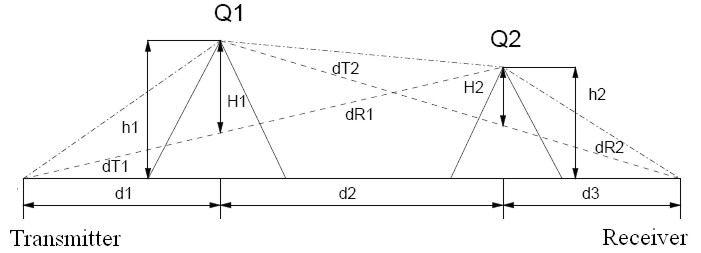
\includegraphics[height=0.3\textwidth]{Immagini/epsteinpeterson}
\caption{Il segnale si propaga fino all'ostacolo successivo che poi diventa la nuova sorgente, così fino al dispositivo ricevitore.}
\label{img:epsteinpeterson}
\end{figure}

\subsubsection{Bilancio di radiocollegamento}
\label{cap:bilancio}
Per bilancio di radiocollegamento, in inglese \emph{Link Budget}, si intende l'insieme dei guadagni e delle perdite dall'apparato
trasmettitore, attraverso il mezzo (spazio libero, cavo, fibra, \ldots), fino all'apparato ricevitore, in un sistema di telecomunicazioni. \\
Essa rappresenta l'attenuazione dovuta alla propagazione del segnale trasmesso, così come i guadagni di antenna le perdite di linea o 
di altra natura.
I guadagni di canale casualmente variabili come il fading sono presi in considerazione aggiungendo qualche margine a seconda della gravità 
prevista dei suoi effetti.
\\[1cm]
Un semplice esempio di equazione di bilancio di radiocollegamento è come questa:
\begin{align*}
Potenza Ricevuta [dBm] &= Potenza Trasmessa [dBm] &+ \\
&+ Guadagni [dB] &+ \\
&- Perdite [dB]
\end{align*}

Per sistemi \ac{LOS} la prima causa di perdita è la diminuzione della potenza del segnale dovuta alla propagazione uniforme, proporzionale
al quadrato inverso della distanza. Nel calcolo della potenza ricevuta si devono considerare alcuni fattori e semplificazioni che rendono
il calcolo più agevole:
\begin{itemize}
\item Le antenne trasmittenti sono per la maggior parte non isotropiche.
\item Antenne omnidirezionali sono molto rare nelle telecomunicazioni, quindi in ogni equazione di bilancio di radiocollegamento si deve
considerare il guadagno di antenna.
\item  Le antenne trasmittenti concentrano la potenza del segnale nella direzione in cui sono rivolte le antenne riceventi.
\item Il termine della lunghezza d'onda è spesso considerato parte dell'equazione della perdita nello spazio libero. 
Questa riduzione di complessità è accettabile per sistemi di comunicazione terrestri, considerando percorsi \ac{LOS}.
\item Si considera la propagazione dell'onda portante indipendente dalla lunghezza d'onda, questo è giustificato legge della 
conservazione dell'energia, la quale richiede che il campo elettrico diminuisca in potenza come il quadrato della distanza 
indipendentemente dalla frequenza (nello spazio libero).
\item Il cablaggio tra le radio e le antenne può introdurre significative perdite supplementari.
\item Effetto doppler induce perdita di potenza nel ricevitore. 
\end{itemize}
\subsubsection{Equazione}
\[
 P_{Rx} = P_{Tx} + G_{Tx} - L_{Tx} - L_{FS} - L_{M} + G_{Rx} - L_{Rx}
\]
dove \\
$P_{Rx}$ è la potenza ricevuta \\
$P_{Tx}$ è la potenza trasmessa \\
$G_{Tx}$ è il guadagno dell'antenna \\
$L_{Tx}$ sono le perdite del trasmettitore \\
$L_{FS}$ è la perdita nello spazio libero \\
$L_{M}$ indica perdite varie (margine di fading, polarizzazione non corrispondente, \ldots) \\
$G_{Rx}$ è il guadagno dell'antenna ricevente \\
$L_{Rx}$ sono le perdite del ricevitore \\

\subsubsection{Margine di radiocollegamento}
Per compensare il fenomeno del fading si cerca di aumentare il livello di potenza del segnale in uscita di una quantità detta
\emph{margine di fading $M_{F}$} in modo da mantenere per tutta la durata del collegamento un sufficiente \ac{SNR}. \\
Il valore di $M_{F}$ necessario a garantire una prefissata affidabilità del collegamento è valutato in base ad analisi teoriche e 
sperimentali. Per esempio per comunicazioni satellitari, che operano a $10GHz$ è sufficiente un margine di fading $M_{F} = 6 dB$. \\
Per i collegamenti in ponte radio terrestri si suppone che il fading segua una \emph{distribuzione di Rayleigh}, si definisce la 
disponibilità del collegamento come:
\[
 D = e^{-\frac{P_{min}}{P_{R}}}
\]
dove $P_{min}$ è la potenza minima che il ricevitore è in grado di riconoscere e $P_{R}$ è la potenza effettivamente ricevuta, il margine
di fading si ottiene quindi dalla relazione:
\[
 (M_{F})_{dB} = -10\log{\left | \ln{D} \right | }
\]

\begin{table}[h]\footnotesize
\caption{Valori caratteristici del margine di radiocollegamento.}
\label{tab:margine}
\begin{tabularx}{\textwidth}{XX}
\toprule
Disponibilità D del collegamento (\%) & Margine di fading $M_{F}$ (dB) \\
\midrule
90 & 10 \\
99 & 20 \\
99.9 & 30 \\
99.99 & 40 \\
99.999 & 50 \\
\bottomrule
\end{tabularx}
\end{table}

Nel caso considerato, la somma tra $P_{Tx}$, $G_{Tx}$ e perdita dei cavi è detta \ac{EIRP} ed è pari a circa $62 dBm$. Si considera, inoltre,
la \emph{sensitività del ricevitore}, la quale è data dalla somma tra cifra di rumore, rumore termico e \ac{SINR}, la somma di questi
tre fattori è circa $106.4 dBm$. \\
Infine è aggiunto il margine di interferenza, il guadagno dell'antenna ricevente $G_{Rx}$ e il controllo di canale. \\
Nel simulatore è stata fatta variare la potenza trasmessa per prolungare la durata della batteria del velivolo, l'attenuazione massima 
in grado di riconoscere il ricevitore è di $163.5 dBm$ per potenza trasmessa di $46 dBm$, $141.5 dBm$ per $24 dBm$ trasmessi e $137.5 dBm$
per $20 dBm$ trasmessi.

\section{Analisi di Copertura della Rete}
\label{cap:copertura}
Una volta modellato il terreno e gli ostacoli come descritto nel capitolo \ref{cap:dem}, si è cercato di analizzare la copertura 
del sistema \ac{LTE} montata sull'\ac{UAV}.

\subsection{Calcolo dell'area coperta}
L'attenuazione è stata calcolata in ogni pixel valido della mappa, per pixel valido si intende qualsiasi pixel che non rappresenti un 
ostacolo. \\
Per ottenere l'attenuazione è stato sviluppato un script Matlab interagente con quello descritto nel capitolo \ref{cap:dem}, questo 
programma riceve in \emph{input} i dati della mappa come altezze del terreno, posizione e altezza degli ostacoli e le coordinate e l'altezza
dell'\ac{UAV}. Una volta lanciato lo script si otterranno tre matrici delle stesse dimensioni della mappa:
\begin{itemize}
\item La prima restituisce l'attenuazione \emph{free space} pixel $\times$ pixel.
\item La seconda contiene l'attenuazione \emph{supplementare} dovuta alla presenza di ostacoli.
\item La terza è la somma delle prime due e rappresenta l'attenuazione totale pixel $\times$ pixel.
\end{itemize}

\subsubsection{Ostacoli tra elicottero ed utente}
L'individuazione di tutti gli ostacoli che si frappongono tra elicottero ed utente, su una linea retta, permette di calcolare la 
diffrazione del segnale in modo da poter applicare quanto visto nel paragrafo \ref{sec:epsteinpeterson}. \\
Questo tipo di problema si traduce nell'applicazione di concetti di base di geometria. Per prima cosa è stato suddiviso lo spazio in 
due aree individuate dal valore del coefficiente angolare della retta passante per elicottero ed utente: come mostrato nella figura
\ref{img:areagriglia} nelle zone in celeste il coefficiente angolare della retta passante per due punti varia tra -1 e +1 altrimenti la 
retta passa per la zona arancione. Il sistema di riferimento è centrato sulle coordinate dell'elicottero.
\begin{figure}[h]
\centering
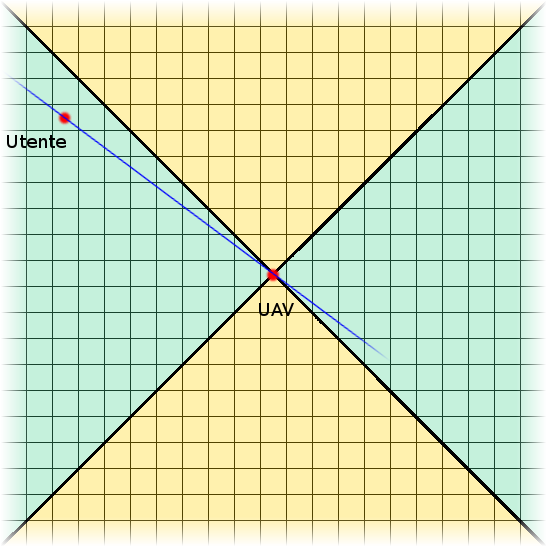
\includegraphics[height=0.7\textwidth]{Immagini/areagriglia}
\caption{Suddivisione dell'area da analizzare.}
\label{img:areagriglia}
\end{figure}
Per individuare gli ostacoli che incontrano la retta è stato campionato l'asse delle ascisse, o delle ordinate a seconda della zona, in
modo da controllare tutti i punti intermedi tra un pixel e l'altro. Come $x$ si prende una lista di valori che va dalla $x_{e}$, ascissa
dell'elicottero, fino alla $x_{u}$, ascissa dell'utente. Da questa lista di coordinate è facile ottenere i rispettivi valori delle 
ordinate:
\begin{equation}
\textbf{y} = y_{u} + \frac{y_{e}-y_{u}}{x_{e}-x_{u}}(\textbf{x}-x_{u})
\label{eq:rettaduepunti}
\end{equation}
dove $\textbf{x}$ e $\textbf{y}$ sono vettori contenenti la lista di coordinate. \\
La suddivisione in zone è molto importante, se si campionasse solo lungo l'asse delle ascisse, per rette quasi verticali si avrebbero 
pochi valori da controllare, così invece, è possibile campionare le rette sfruttando tutta la loro lunghezza. \\
Con questo tipo di approccio si evidenzierà una zona limitrofa alla retta (regione in giallino), dove sarà necessario controllare la 
presenza degli ostacoli:
\begin{figure}[h]
\centering
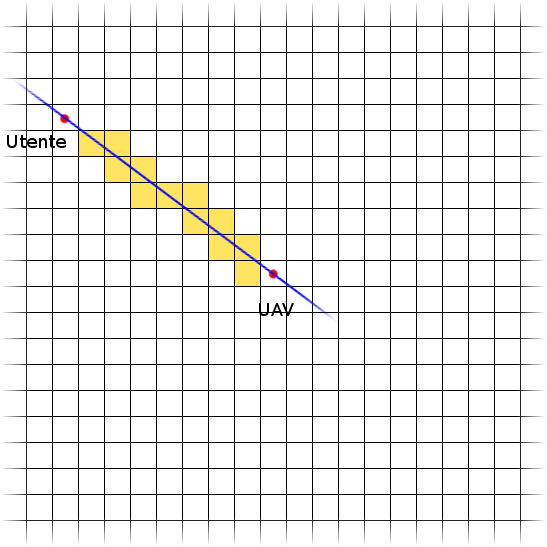
\includegraphics[height=0.7\textwidth]{Immagini/quadretti}
\caption{Pixel passanti per la retta.}
\label{img:quadretti}
\end{figure}
Ottenute tutti i pixel per cui passa la retta, si deve prendere la parte intera di ogni coordinata per ottenere il pixel 
corrispondente; a questo punto si deve controllare se ogni pixel faccia parte di un ostacolo: si prende la maschera degli ostacoli 
(\ref{img:comask}) e si controlla se il pixel appartenga o meno all'ostacolo. \\
Evidenziati gli ostacoli dall'area in giallino della figura \ref{img:quadretti} è necessario distinguere gli ostacoli in base alla loro
altezza; il modello di Epstein-Peterson, infatti, permette di modellare un ostacolo come se fosse una lama di coltello, quindi se più
pixel vicini hanno la stessa altezza faranno parte dello stesso ostacolo e nella lista degli ostacoli tra elicottero ed utente dovranno
essere considerati come uno solo.
Il modello di Epstein-Peterson sulla diffrazione dovuta ad ostacoli multipli è definito su una retta, l'area in giallino, invece, definisce
una zona limitrofa alla retta tra elicottero ed utente: si devono quindi proiettare le coordinate degli ostacoli sulla retta. \\
Per implementare ed automatizzare la proiezione del pixel sulla retta sono stati utilizzati dei semplici concetti di geometria analitica;
dati tre punti, coordinate dell'elicottero, coordinate dell'utente e coordinate dell'ostacolo si devono calcolare le coordinate della 
proiezione in funzione di questi tre punti:
\begin{align*}
E &= (x_{e},y_{e}) \\
U &= (x_{u},y_{u}) \\
O &= (x_{o},y_{o}) \\
\end{align*}
Si considera la retta (\ref{eq:rettaduepunti}) passante per $E$ ed $U$, la perpendicolare passante per $O$ avrà equazione:
\begin{equation}
y = y_{o} - \frac{x_{e}-x_{u}}{y_{e}-y_{u}}(x-x_{o})
\label{eq:perpendicolareost}
\end{equation}
L'intersezione della retta \ref{eq:rettaduepunti} con la \ref{eq:perpendicolareost}, mi darà le coordinate della proiezione dell'ostacolo
sulla retta, i punti in verde nell'immagine \ref{img:proiezioni}.
\begin{align*}
x &= \frac{(y_{o}-y_{e}) (y_{u}-y_{e}) (x_{u}-x_{e}) + x_{o} (x_{u}-x_{e})^{2} + x_{e} (y_{u}-y_{e})^{2}}
	  {(y_{u}-y_{e})^{2} + (x_{u}-x_{e})^{2}} \\
y &= y_{e} + (y_{u}-y_{e}) \frac{(y_{o}-y_{e}) (y_{u}-y_{e}) + (x_{o}-x_{e}) (x_{u}-x_{e})}
			        {(y_{u}-y_{e})^{2} + (x_{u}-x_{e})^{2}}
\end{align*}
\begin{figure}[h]
\centering
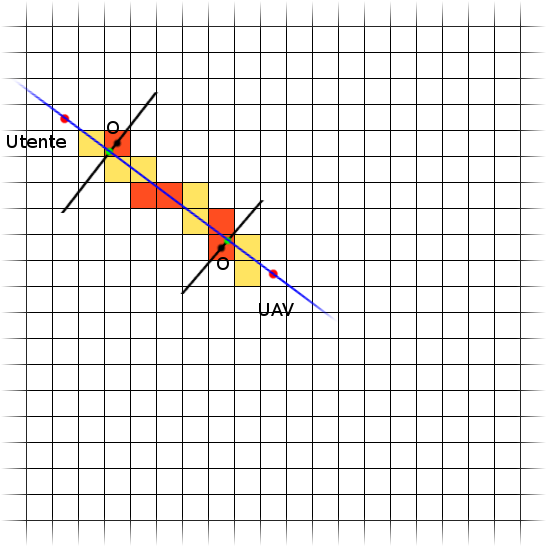
\includegraphics[height=0.7\textwidth]{Immagini/proiezioni}
\caption{Proiezioni degli ostacoli sulla retta.}
\label{img:proiezioni}
\end{figure}
Dopo aver calcolato la proiezione di ogni ostacolo sulla retta si ottiene una lista di ostacoli tra elicottero ed utente, adesso è possibile
applicare il modello di Epstein-Peterson per calcolare l'attenuazione dovuta alla diffrazione.

\subsubsection{Parametro di diffrazione}
Il modello di Epstein-Peterson si riduce a calcolare l'attenuazione dovuta ad un singolo ostacolo ed a replicare il calcolo ostacolo per 
ostacolo, Quindi il problema del calcolo della diffrazione per ostacolo multiplo può essere semplificato al calcolo per ostacolo singolo. \\
Partendo quindi dalla lista di ostacoli tra elicottero ed utente si calcola la distanza tra elicottero e primo ostacolo e tra ostacolo 
ed utente, infine si calcola il franco e si applica la formula \ref{eq:parametrodiffrazione} per ottenere il \emph{parametro di diffrazione}.

\subsubsection{Attenuazione dovuta alla diffrazione}
Il calcolo dell'attenuazione pixel $\times$ pixel è quasi terminato, adesso si ha per ogni pixel il parametro di diffrazione dovuto agli
ostacoli che si frappongono tra elicottero ed utente. \\
Il parametro di diffrazione permette di calcolare le due funzioni integralcoseno ed integralseno, le quali sottratte tra loro restituiscono
l'integrale complesso di Fresnel (\ref{eq:integralefresnel}).
Quest'ultimo valore permette di ottenere il fattore di diffrazione $v$, il quale, calcolato in dB, dà l'attenuazione nel determinato
pixel. \\
Ripetendo il processo per ogni pixel della matrice, si otterranno le matrici con l'attenuazione (free space, supplementare e totale)
calcolata per ogni pixel.


\subsubsection{Calcolo del raggio di copertura}
Il calcolo del raggio di copertura permette di evidenziare l'area coperta dal segnale trasmesso dall'\ac{UAV}, in base all'attenuazione
massima tollerabile dal ricevitore. \\
Per il calcolo dell'attenuazione è stata seguita la procedura descritta nel capitolo \ref{cap:bilancio}, una volta ottenuta questa soglia
si procede a confrontarla con l'attenuazione calcolata in ogni pixel, se quest'ultima è superiore allora si suppone che quel pixel non
sia coperto dal segnale trasmesso dall'\ac{UAV}.
A questo punto il calcolo del raggio si semplifica in una semplice distanza tra due punti:
\begin{figure}[h]
\centering
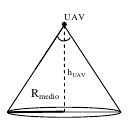
\includegraphics[height=0.3\textwidth]{Immagini/raggio}
\caption{Il raggio è la distanza sul piano tra \ac{UAV} ed utente coperto da segnale.}
\label{img:raggio}
\end{figure}
Il raggio viene quindi calcolato per ogni punto coperto, il risultato è una matrice contenente le distanze tra elicottero ed utente. \\

Una volta calcolato il raggio di copertura pixel $\times$ pixel è possibile calcolare il raggio medio di copertura come la media 
aritmetica tra i raggi ottenuti, così facendo si otterrà un'area circolare dove la maggior parte del segnale sarà concentrato. \\
Oltre al raggio medio di copertura, un indice più veritiero della copertura totale del segnale è dato dai percentili del raggio di 
copertura; presi tutti i raggi punto per punto è stato calcolato l'$80^o$ percentile in modo da rappresentare il raggio che contiene 
l'$80\%$ dell'area coperta da segnale.

\subsubsection{Miglioramento di copertura dell'area}
Al fine di migliorare i settori esclusi dai calcoli precedenti, dove l'attenuazione del segnale è superiore alla massima consentita, sarà
possibile proseguire secondo due approcci: la variazione della posizione degli \ac{UAV} e l'utilizzo di più \ac{UAV}.
La prima possibilità prevede di far seguire ad un \ac{UAV} un loop sull'area da coprire, in modo da offrire, anche se per una durata 
limitata, ad ogni utente il segnale per poter comunicare nell'area. \\
Con la seconda possibilità si coordineranno più \ac{UAV} a formare una rete a maglie, la cosiddetta rete \emph{mesh}, in modo da poter
coprire un'area molto più estesa. \\ 
Le due possibilità, ovviamente, potrebbero anche coesistere a seconda delle esigenze dei soccorritori, come per esempio per l'espansione
dell'area, il numero di \ac{UAV} a disposizione, \ldots
%\input{Capitoli/dem}
%\input{Capitoli/copertura}
\chapter{Risultati}
\label{cap:risultati}
In questo lavoro di tesi sono stati simulati tre scenari, relativi a tre diverse zone di Roma:
\begin{enumerate}
 \item Il territorio attorno alle facoltà di Ingegneria, Economia e Lettere dell'Università di Roma Tor Vergata.
 \item La zona tra la stazione di Roma Termini e il Colosseo.
 \item L'area con al centro il Pantheon.
\end{enumerate}
Sono state scelte queste tre aree perché presentano una morfologia particolare, partendo dalla zona dell'Università fino a quella 
del Pantheon si può vedere come l'area urbana e la densità di edifici aumenti. Anche le aree verdi passano dalla zona attorno 
all'Università, al Parco Del Colle Oppio, fino alla zona del Pantheon piena di edifici. \\
In tutte le simulazioni l'\ac{UAV} è stato posto al centro dell'area e l'antenna trasmittente è stata supposta un dipolo omnidirezionale. \\
Durante le simulazioni è stata fatta variare la potenza trasmessa dall'apparato \ac{LTE} dell'\ac{UAV} per fare in modo di gestire un 
eventuale risparmio energetico al fine di prolungare la durata della batteria del velivolo. \\
Si ricorda che ogni area ha una superficie di $1km^2$ con una risoluzione di $200 \times 200 pixel$.
Per ognuna di queste tre zone sono stati calcolati questi parametri:
\begin{itemize}
 \item Attenuazione totale, calcolata $pixel \times pixel$.
 \item Raggio medio di copertura.
 \item Raggio medio all'$80^o$ percentile.
\end{itemize}

\section*{Confronto tra le tre zone}
Nella tabella \ref{tab:confrontozone} sono rappresentati i raggi di copertura per ogni zona al variare della potenza, a potenza massima è
molto evidente come il raggio diminuisca con l'aumento della densità urbana.
 \begin{table}[h]\footnotesize
  \caption{Raggi di copertura nelle tre zone al variare della potenza trasmessa.}
  \label{tab:confrontozone}
  \begin{tabularx}{\textwidth}{lXXX}
    \toprule
      & $Ptx = 46dBm$ & $Ptx = 24dBm$ & $Ptx = 20dBm$ \\
    \midrule
      Zona 1 & 506.1867 m & 504.2321 m & 503.3140 m \\
      Zona 2 & 490 m & 392.0459 m & 365.2773 m \\
      Zona 3& 473.0486 m & 408.0747 m & 371.9339 m \\
    \bottomrule
    \end{tabularx}
  \end{table}

\newpage
\section{Area facoltà di Ingegneria, Economia e Lettere}
L'area attorno alle facoltà di Ingegneria, Economia e Lettere dell'Università di Roma Tor Vergata, sono libere da ostacoli.
Gli unici edifici presenti sono quelli dei dipartimenti di Ingegneria (Ingegneria dell'Informazione, Ingegneria Industriale ed Ingegneria
Civile), gli edifici delle facoltà di Lettere e di Economia. 
Il resto, tra parcheggi ed aree verdi, è tutto spazio libero disponibile per l'utente, ci si aspetta quindi che l'area coperta dal segnale
sia la maggior parte se non tutta quanta. \\
Dai calcoli del raggio si ottiene che l'area coperta è circa il $80\%$ di quella totale, ma dato che i calcoli si basano sul calcolo dell'
$80^o$ percentile, risulta che è coperto il $100\%$ dell'area. L'area coperta diminuisce di poco anche a potenza minima.

\begin{figure}[!h]
\centering
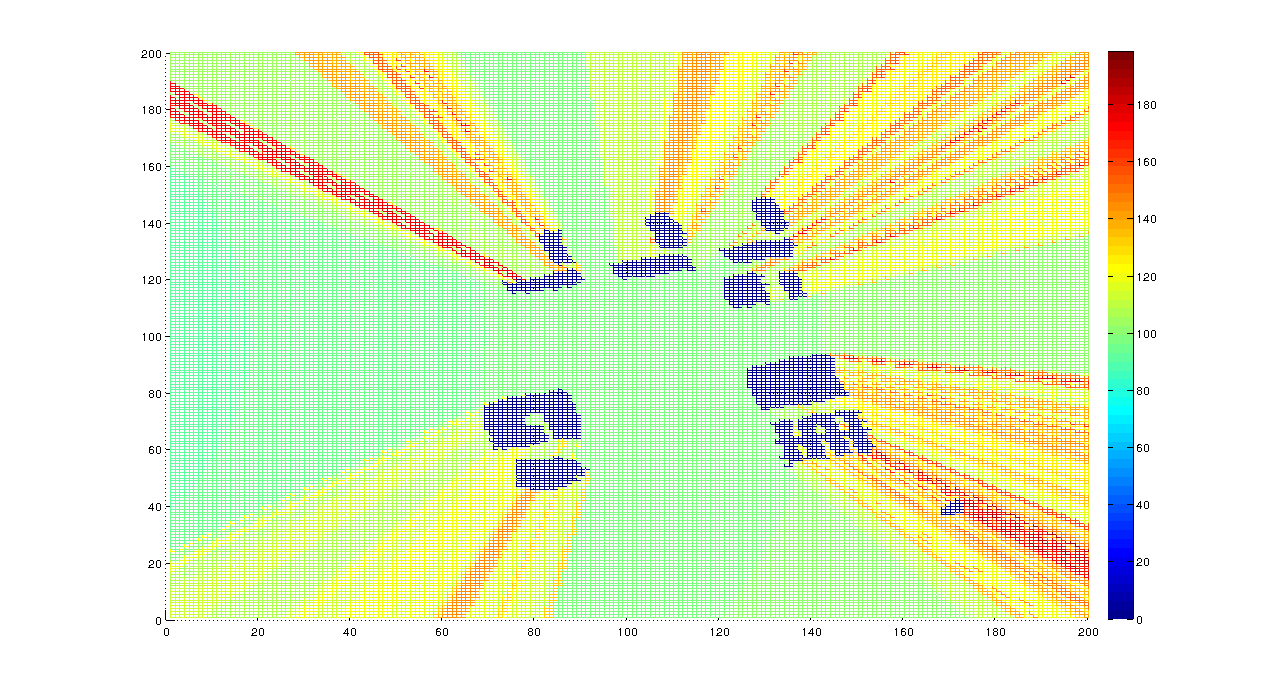
\includegraphics[height=0.5\textwidth]{Immagini/TorVergataIng/attenuazione}
\caption{Attenuazione nella zona delle facoltà di Ingegneria, Economia e Lettere dell'Università di Roma Tor Vergata con potenza
trasmessa pari a $46dBm$. \\
Il raggio medio è pari a $388.3664 m$.\\
Il raggio medio calcolato all'$80^o$ percentile è di $506.1867 m$.}
\label{img:atting}
\end{figure}

\begin{figure}
\centering
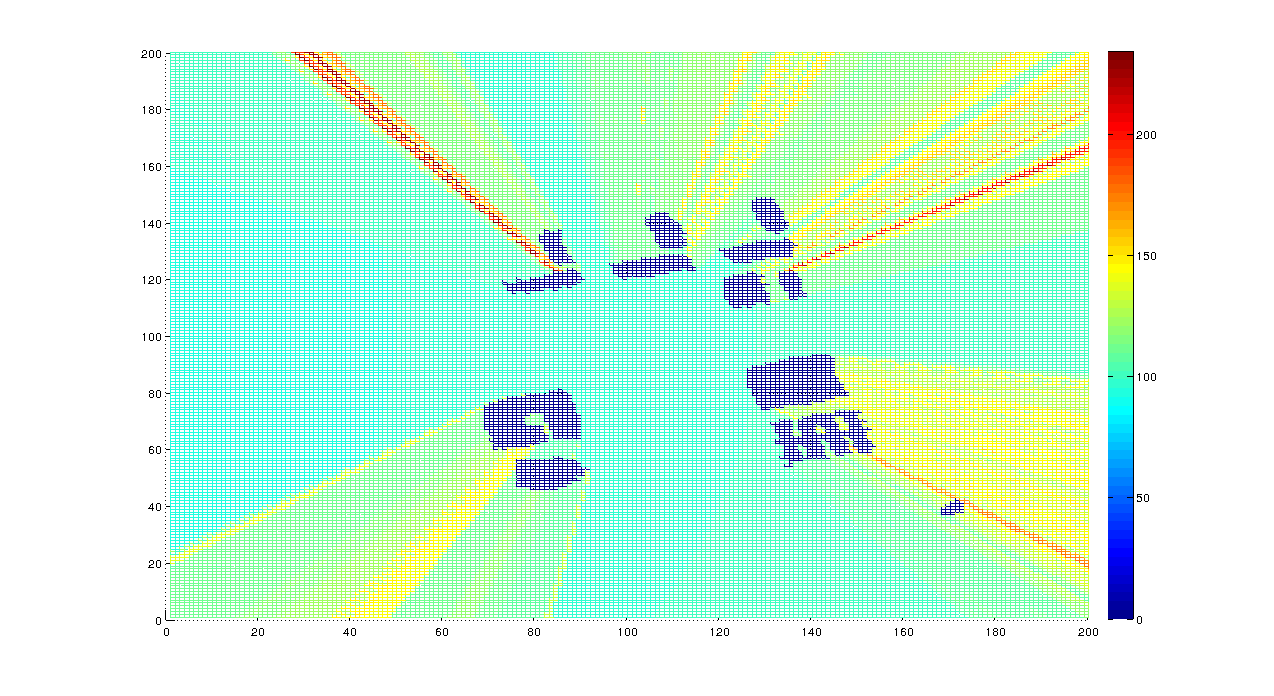
\includegraphics[height=0.5\textwidth]{Immagini/TorVergataIng/attenuazione_pico}
\caption{Attenuazione nella zona delle facoltà di Ingegneria, Economia e Lettere dell'Università di Roma Tor Vergata con potenza
trasmessa pari a $24dBm$. \\
Il raggio medio è pari a $386.0185 m$. \\
Il raggio medio calcolato all'$80^o$ percentile è di $504.2321 m$.}
\label{img:attingpico}
\end{figure}

\begin{figure}
\centering
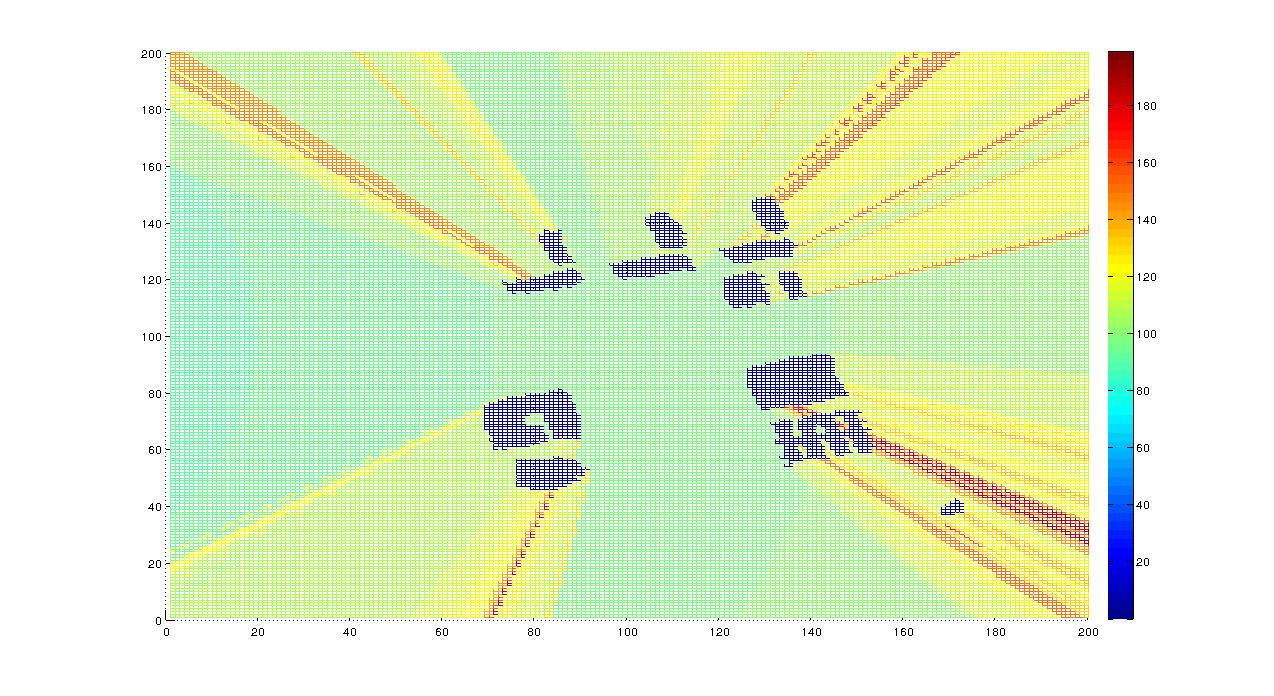
\includegraphics[height=0.5\textwidth]{Immagini/TorVergataIng/attenuazione_femto}
\caption{Attenuazione nella zona delle facoltà di Ingegneria, Economia e Lettere dell'Università di Roma Tor Vergata con potenza
trasmessa pari a $20dBm$. \\
Il raggio medio è pari a $384.704 m$. \\
Il raggio medio calcolato all'$80^o$ percentile è di $503.3140 m$.}
\label{img:attingfemto}
\end{figure}

\newpage
\section{Area tra Roma Termini e Colosseo}
Nella zona tra la stazione di Roma Termini e il Colosseo l'ambiente è una via di mezzo tra urbano e spazio libero, si va dal Parco Del
Colle Oppio fino alla zona urbana attorno a Roma Termini. \\
Con la massima potenza trasmessa si riesce a coprire il $75\%$ dell'area, quindi sempre riferendosi al percentile $80$ si capisce che la
copertura è quasi totale, a potenza minima, invece, la copertura scende al $40\%$ quindi l'area coperta è circa il $50\%$.

\begin{figure}[!h]
\centering
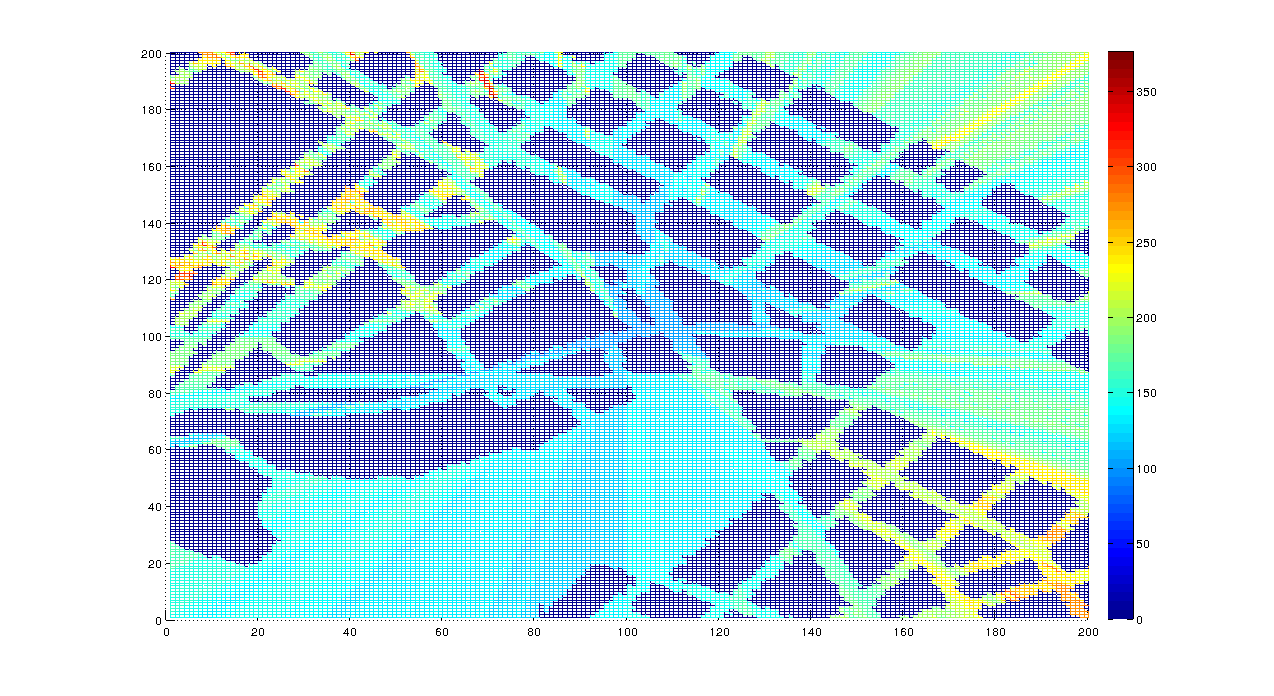
\includegraphics[height=0.5\textwidth]{Immagini/ColleOppio/attenuazione}
\caption{Attenuazione nella zona tra Colle Oppio e Roma Termini con potenza trasmessa pari a $46dBm$. \\
Il raggio medio è pari a $363.9597 m$.\\
Il raggio medio calcolato all'$80^o$ percentile è di $490 m$.}
\label{img:attcolleoppio}
\end{figure}

\begin{figure}
\centering
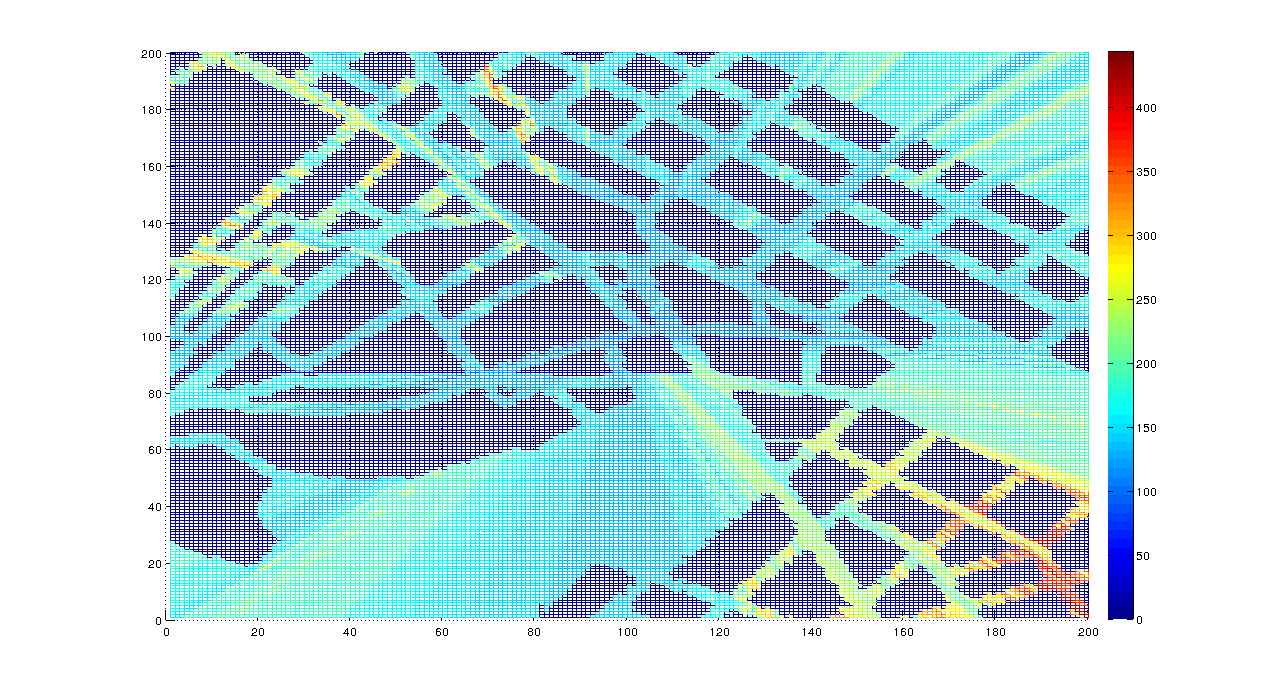
\includegraphics[height=0.5\textwidth]{Immagini/ColleOppio/attenuazione_pico}
\caption{Attenuazione nella zona tra Colle Oppio e Roma Termini con potenza trasmessa pari a $24dBm$. \\
Il raggio medio è pari a $282.0619 m$.\\
Il raggio medio calcolato all'$80^o$ percentile è di $392.0459 m$.}
\label{img:attcolleoppiopico}
\end{figure}

\begin{figure}
\centering
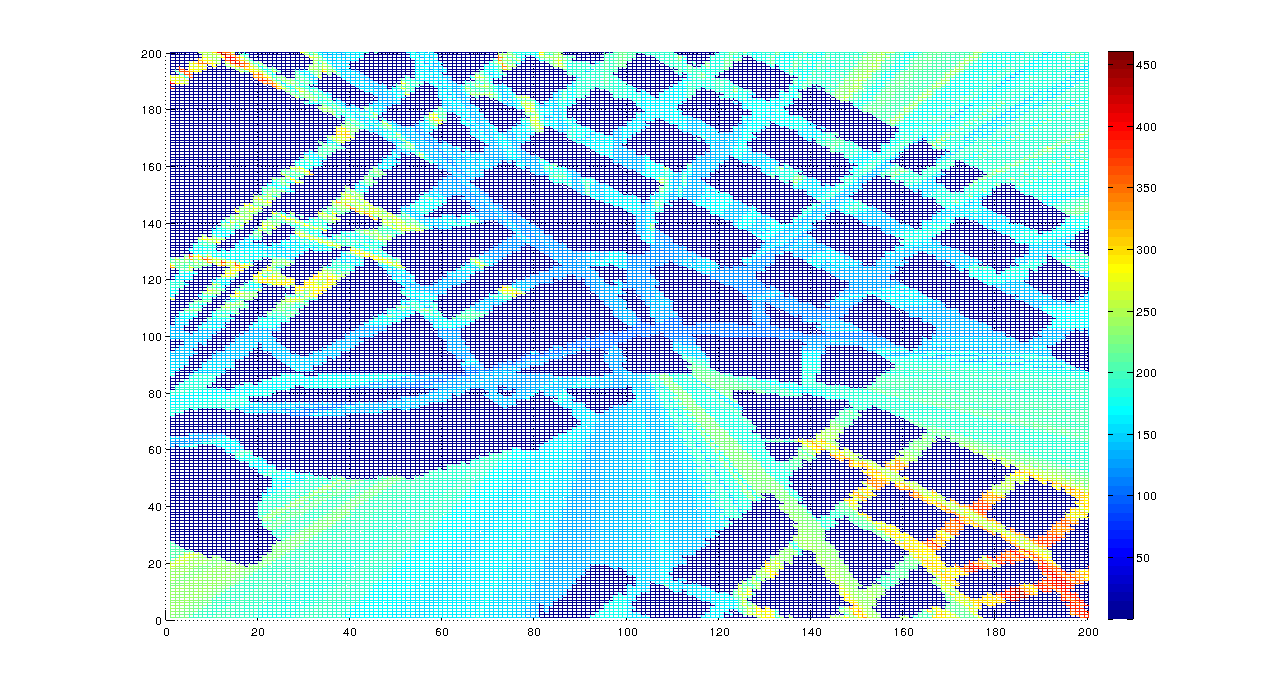
\includegraphics[height=0.5\textwidth]{Immagini/ColleOppio/attenuazione_femto}
\caption{Attenuazione nella zona tra Colle Oppio e Roma Termini con potenza trasmessa pari a $20dBm$. \\
Il raggio medio è pari a $256.2801 m$.\\
Il raggio medio calcolato all'$80^o$ percentile è di $365.2773 m$.}
\label{img:attcolleoppiofemto}
\end{figure}

\newpage
\section{Area Pantheon}
Nell'area urbana dove è ubicato il Pantheon, l'ambiente urbano è predominante è quello urbano, non ci sono aree libere e l'utente può
trovarsi solo lungo le strade. \\
A potenza massima il raggio all'$80^o$ percentile copre un'area pari al $70\%$, normalizzando si ottiene che l'area coperta è circa 
l'$87\%$, al diminuire della potenza l'area normalizzata coperta arriva a circa un $55\%$

\begin{figure}[!h]
\centering
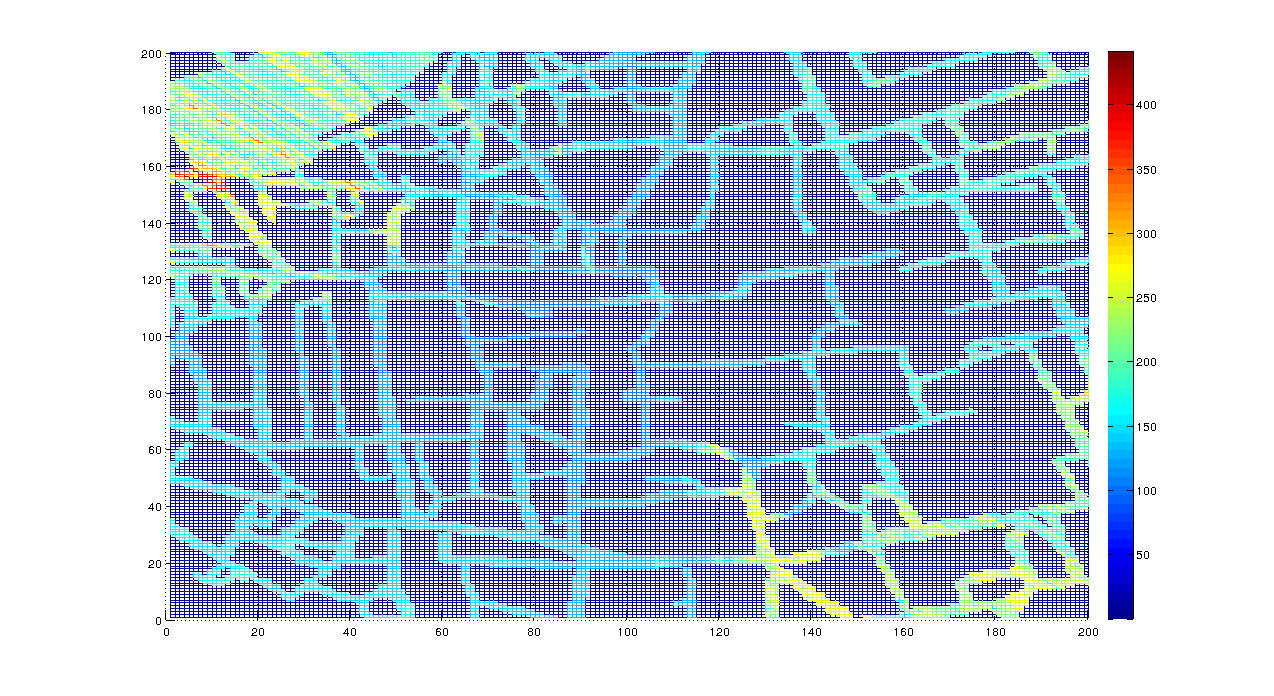
\includegraphics[height=0.5\textwidth]{Immagini/Pantheon/attenuazione}
\caption{Attenuazione nell'area del Pantheon con potenza trasmessa pari a $46dBm$. \\
Il raggio medio è pari a $348.2113 m$.\\
Il raggio medio calcolato all'$80^o$ percentile è di $473.0486 m$.}
\label{img:attpantheon}
\end{figure}

\begin{figure}
\centering
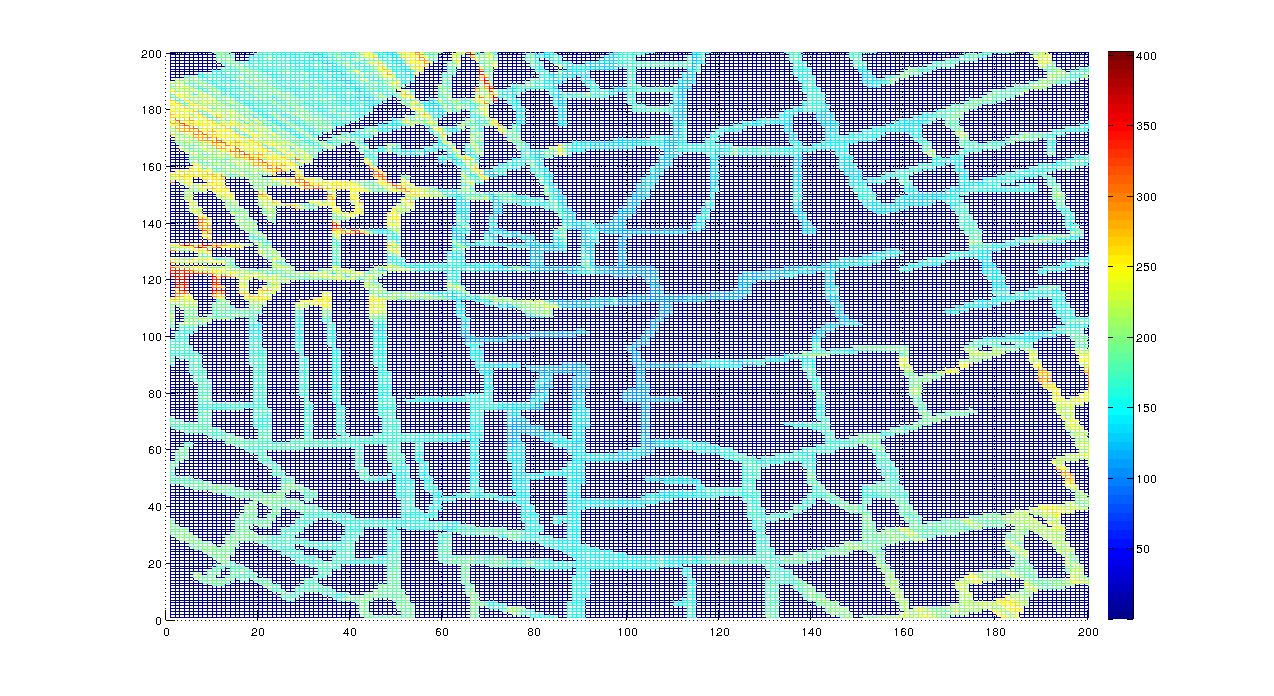
\includegraphics[height=0.5\textwidth]{Immagini/Pantheon/attenuazione_pico}
\caption{Attenuazione nell'area del Pantheon con potenza trasmessa pari a $24dBm$. \\
Il raggio medio è pari a $294.3916 m$.\\
Il raggio medio calcolato all'$80^o$ percentile è di $408.0747 m$.}
\label{img:attpantheonpico}
\end{figure}

\begin{figure}
\centering
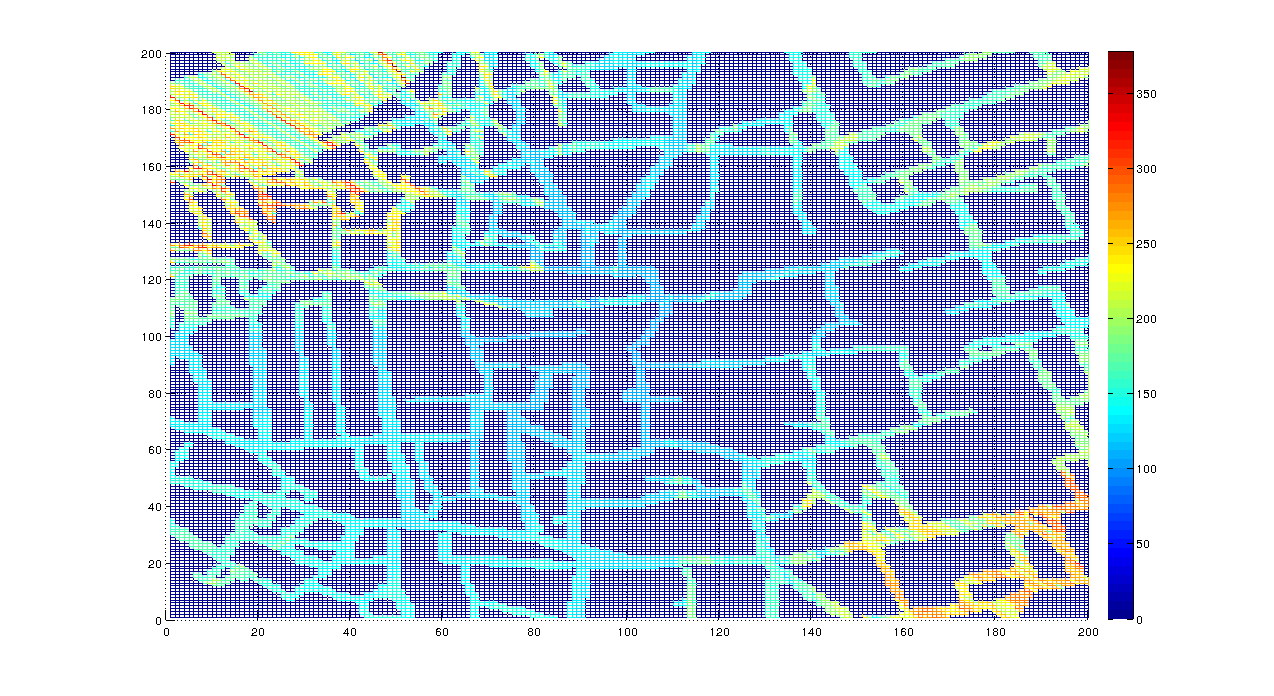
\includegraphics[height=0.5\textwidth]{Immagini/Pantheon/attenuazione_femto}
\caption{Attenuazione nell'area del Pantheon con potenza trasmessa pari a $20dBm$. \\
Il raggio medio è pari a $242.1427 m$.\\
Il raggio medio calcolato all'$80^o$ percentile è di $371.9339 m$.}
\label{img:attpantheonfemto}
\end{figure}
%\appendix
%\input{Capitoli/Dolor}
% *****************************************************************
% Materiale finale
%******************************************************************
\input{MaterialeInizialeFinale/Bibliografia}
%\input{MaterialeInizialeFinale/Dichiarazione}
\end{document}
